\documentclass[11pt]{article}

\usepackage[margin=1in]{geometry}
\usepackage[T1]{fontenc}
\usepackage{lmodern}
\usepackage{amsmath,amssymb}
\usepackage{graphicx}
\usepackage{booktabs}
\usepackage{longtable}
\usepackage{adjustbox}
\usepackage{array}
\usepackage{float}
\usepackage{caption}
\usepackage{subcaption}
\usepackage{xcolor}
\usepackage{amssymb}
\usepackage{pgfplots}
\pgfplotsset{compat=1.16}
\usepackage[hidelinks]{hyperref}

\graphicspath{{figures/}}
\newcommand{\var}[1]{\texttt{#1}}

\title{\textbf{Learning to Listen:}\\[4pt]
A Cost-Aware Ablation Study of a Perch-Distilled Sound Event Detection Network
for Multi-Taxon Passive Acoustic Monitoring}
\author{Saurav Bellam}
\date{October 2026}

\begin{document}
\maketitle

% ===========================================================================
\begin{abstract}
We want the cheapest species classifier that still works well enough to run
continuously on site for passive acoustic monitoring of the Brazilian
Pantanal. We study a ResNet-18 sound event detection (SED) network that
classifies 234 bird, amphibian, insect, mammal and reptile classes from 5\,s
audio windows, using the BirdCLEF~2026 data. The full model combines several
components: 3-channel log-mel/delta/delta-delta input, a GeM-frequency +
attention-over-time SED head, distillation of embeddings from Google's Perch~v2
model with a stop-gradient on the classifier, Perch-localised pseudo-labels for
focal recordings and unlabelled soundscapes, mixup, SpecAugment and rare-class
upsampling. Each component was removed one at a time (11 training ablations).
We also evaluated two baselines (a plain pooled ResNet-18 and a frozen Perch
attention probe) and six post-processing variants that need no retraining.
Every variant was scored on 13 metrics and benchmarked for inference cost.

On 3-fold, pooled out-of-fold evaluation over labelled soundscape windows (site
S22 excluded), the full model reaches a macro ROC-AUC of 0.7142. Two simpler
models score higher: the plain ResNet-18 baseline reaches 0.7571, and removing
the pseudo-labelled soundscapes reaches 0.7742 while cutting expected
calibration error from 0.184 to 0.003. Thirteen of 21 pre-registered hypotheses
were supported. The ones that failed were about the expensive ideas:
distillation, pseudo-labelling, GeM pooling, and the Perch teacher beating the
student on rare species. Every CNN variant costs the same to run (11.7\,M
parameters, 5.9\,GFLOPs, about 82\,ms per window on one CPU thread, 61$\times$
real time), so component choices are free at inference and should be judged on
quality alone. Three post-processing steps together (a fold-safe site/hour
prior, temporal smoothing and taxonomy smoothing) raise macro ROC-AUC from
0.7142 to 0.8407 at essentially no inference cost. We report every number the
study produced, give file-level bootstrap uncertainty, and discuss why the
evaluation (16 soundscape files, 44 scorable classes, a 10-epoch budget)
limits how far the rankings can be trusted.
\end{abstract}

\tableofcontents
\newpage

% ===========================================================================
\section{Introduction}

Biodiversity monitoring increasingly relies on \emph{passive acoustic
monitoring} (PAM): autonomous recorders left in the field capture the calls of
birds, frogs, insects and mammals around the clock. The bottleneck is
analysis. A single recorder produces about 17{,}000 five-second windows per
day, far more than any expert can label. The Pantanal of Brazil, the world's
largest tropical wetland (over 150{,}000~km$^2$, with more than 650 bird
species), is a prime example: it is vast, seasonally flooded, under threat
from fire and land-use change, and largely unmonitored.

For a monitoring station the right question is not ``what is the most
accurate model?'' but \emph{``what is the cheapest model that is still good
enough to run 24/7 on site?''} A model that needs a data-centre GPU cannot run
on a solar-powered field box. This study is built around that question. Every
variant is judged on \textbf{quality} (13 metrics covering ranking, detection,
calibration, temporal stability and per-taxon performance) and on
\textbf{cost} (parameters, GFLOPs, and CPU and GPU latency per prediction). A
component earns its place only if its quality gain is worth its cost.

\paragraph{Contributions.}
\begin{enumerate}
  \item A cost-aware pipeline: a ResNet-18 student with an attention SED head,
        distilled offline from the Perch~v2 bioacoustics model, with Perch
        also used to pseudo-label every training window
        (Section~\ref{sec:methods}).
  \item A controlled study of 20 variants: 2 baselines, the full model, 11
        one-change training ablations and 6 post-hoc variants. Each tests a
        hypothesis written down before training (Section~\ref{sec:design}).
  \item A complete report of every metric, per-fold selection statistic,
        learning curve, inference and training cost, and attention
        diagnostic produced by the study, plus file-level bootstrap
        confidence intervals that we added (Section~\ref{sec:results}).
  \item An interpretation of what the evidence supports, what it does not,
        and which configuration we would deploy (Sections~\ref{sec:interp}
        and~\ref{sec:recommend}).
\end{enumerate}

\paragraph{Attribution.}
The SED head, the Perch-distillation scheme with stop-gradient, the
pseudo-labelling system and the site/hour priors are adapted from the
``Model\_1'' and ``Model\_22'' sections of the public Kaggle notebook
\emph{BirdCLEF~2026 EoS.9} by nina2025~\cite{nina2025}. That notebook credits
tuckerarrants' distilled-SED and waveform-cache datasets and the BirdCLEF~2025
first-place SED design by nikitababich. Our changes are a ResNet-18 backbone
in place of EfficientNet-B0 (with the global pool removed so the head sees the
time axis), 3-channel stacked inputs, offline Perch pseudo-labels and
embeddings, precomputed spectrograms, a constant learning rate, the ablation
switches, the evaluation and cost harness, and this analysis.

% ===========================================================================
\section{Data}
\label{sec:data}

\subsection{Sources}
We use the BirdCLEF~2026 competition data~\cite{birdclef}:
\begin{itemize}
  \item \textbf{Focal recordings} (\texttt{train\_audio}, \texttt{train.csv}):
        \textbf{35{,}549} clips from Xeno-canto and iNaturalist, each with a
        primary label and optional secondary labels. Secondary labels are
        present for \textbf{4{,}372} files. Clips are split into
        non-overlapping 5\,s windows, giving \textbf{152{,}198 focal windows}.
  \item \textbf{Labelled soundscapes}: 66 one-minute field recordings, i.e.
        \textbf{792 windows} of 5\,s (12 per file). \textbf{739} windows carry
        at least one label, with \textbf{3{,}122} positive (window, species)
        pairs covering \textbf{75 species}. File names encode the recording
        site and time, e.g.\ \path{BC2026_Train_0001_S08_20250606_030007.ogg}.
  \item \textbf{Unlabelled soundscapes}: \textbf{24{,}000} windows (2{,}000
        one-minute files) used only through pseudo-labels.
  \item \textbf{Taxonomy}: \textbf{234 classes} in the competition's column
        order, each with a scientific name and taxonomic class (Aves,
        Amphibia, Insecta, Mammalia, Reptilia). Insect ``sonotypes'' (labels
        such as \texttt{47158son10}) are acoustic morphotypes without a
        species name.
\end{itemize}

\subsection{Class imbalance}
Figure~\ref{fig:focalhist} shows the number of focal clips per class for all
234 classes. \textbf{28 classes have no focal clips at all}: they can be
learned only from soundscapes. \textbf{64 classes} (including those 28) have
fewer than 20 clips and are called \emph{rare}. 46 have 20--99, and
\textbf{124} have at least 100 and are called \emph{common}. The median is
104.5 clips per class and the maximum 499. The pile-up in the top bin
suggests an upstream cap near 500 clips per class.

\begin{figure}[H]
\centering
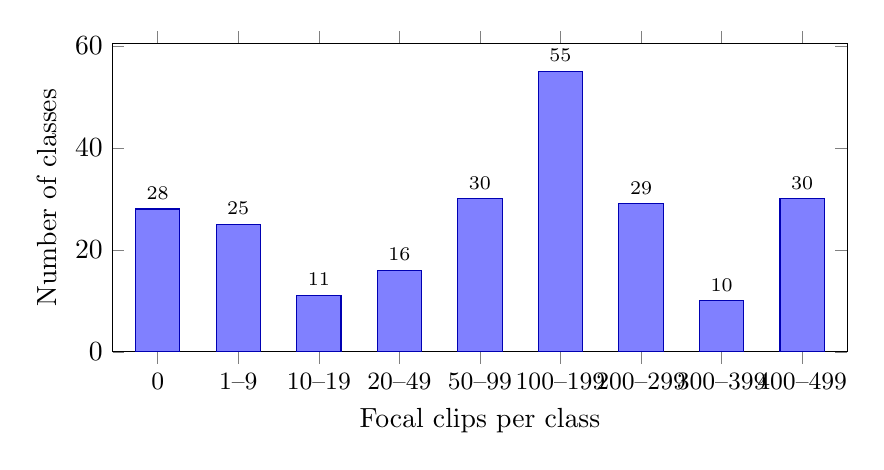
\begin{tikzpicture}
\begin{axis}[ybar, bar width=16pt, width=0.9\linewidth, height=5.5cm,
  ymin=0, ylabel={Number of classes}, xlabel={Focal clips per class},
  symbolic x coords={0,1--9,10--19,20--49,50--99,100--199,200--299,300--399,400--499},
  xtick=data, xticklabel style={font=\small}, nodes near coords,
  nodes near coords style={font=\scriptsize}, enlarge x limits=0.07]
\addplot[fill=blue!50, draw=blue!70!black] coordinates {(0,28) (1--9,25) (10--19,11) (20--49,16)
  (50--99,30) (100--199,55) (200--299,29) (300--399,10) (400--499,30)};
\end{axis}
\end{tikzpicture}
\caption{Focal clips per class for the 234 BirdCLEF~2026 classes (from
\texttt{train\_counts} in the out-of-fold files). The three left bars (64
classes) are the ``rare'' group; classes at or above 100 clips (124) are the
``common'' group.}
\label{fig:focalhist}
\end{figure}

Figure~\ref{fig:classdist} is an earlier view of the same long tail, computed
on the project's curated metadata table (169 labelled classes, counting
primary and secondary labels).

\begin{figure}[H]
\centering
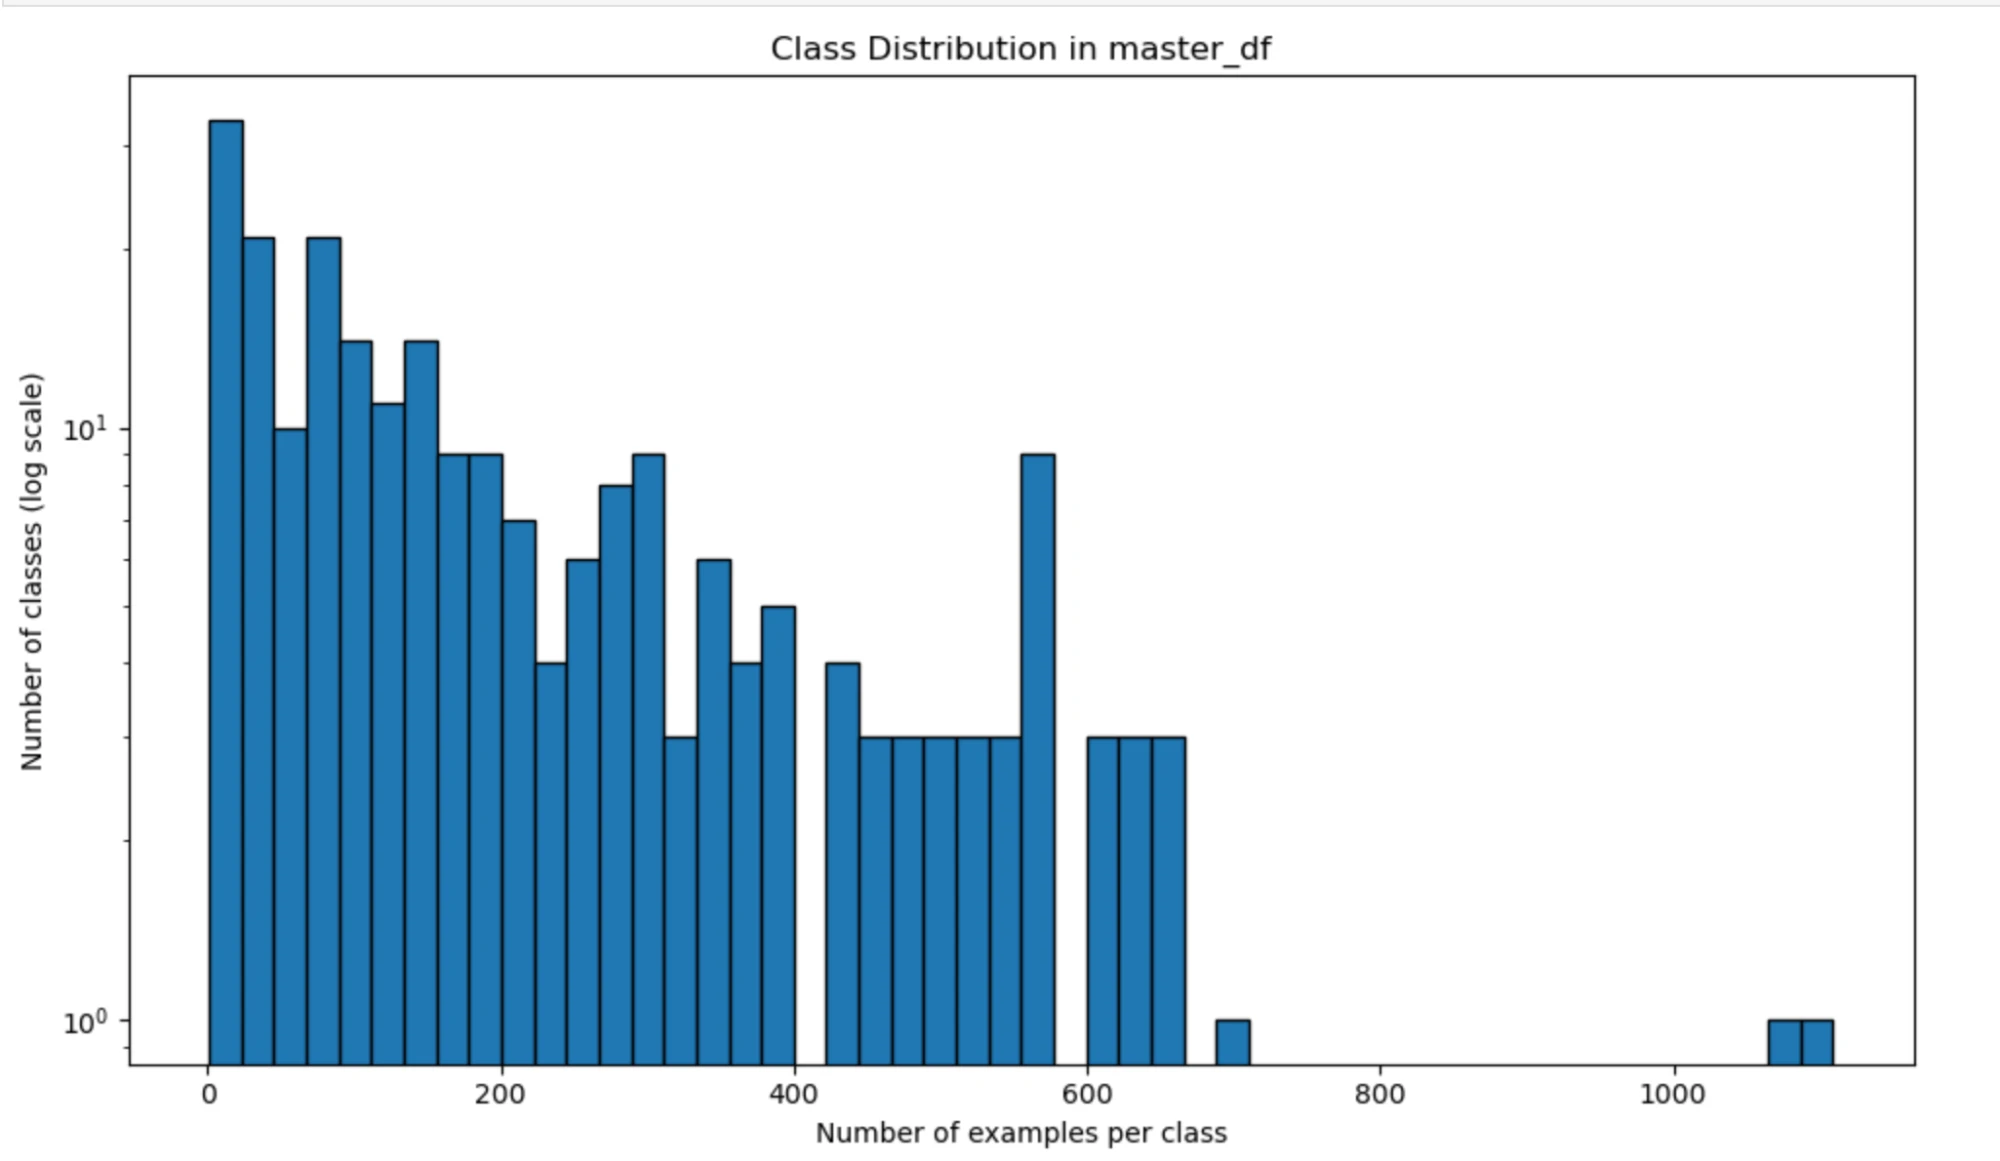
\includegraphics[width=0.75\linewidth]{class_distribution.png}
\caption{Log-scaled histogram of examples per class in the project's curated
metadata table (169 classes). Most classes have only a few dozen examples and a
handful have several hundred.}
\label{fig:classdist}
\end{figure}

\subsection{Cross-validation folds}
Focal clips are split with \texttt{StratifiedKFold} (5 folds, stratified by
primary label, seed 42), giving 7{,}110 clips in each of folds 0--3 and 7{,}109
in fold 4. Labelled soundscape files are split with \texttt{GroupKFold} (5
folds, grouped by file), giving 168 windows in fold 0 and 156 in each of folds
1--4. Because grouping is by file and not by site, the same site can appear in
both training and validation folds. Pseudo-label priors for fold $k$ are fit
without fold-$k$ files (Section~\ref{sec:pseudo}). To fit the compute budget,
\textbf{only folds 0, 1 and 2 were trained} for every variant.

\subsection{Evaluation set}
\label{sec:evalset}
Following the competition notebook, site \textbf{S22} is excluded from scoring
because of known label noise (480 of the 792 soundscape windows; 312 are
non-S22). Predictions exist only for the validation windows of folds 0--2 (480
windows), so the \textbf{evaluation set is the 192 non-S22 windows of folds
0--2}:
\begin{itemize}
  \item 16 soundscape files from 8 sites (S03, S08, S09, S13, S15, S18, S19,
        S23);
  \item 580 positive (window, class) pairs, i.e.\ 3.02 labels per window;
  \item \textbf{44 scorable classes} (at least one positive and one
        negative), with a median of 12 positive windows per class (minimum 1,
        maximum 60) and a mean prevalence of 0.069;
  \item 26 of the 44 scorable classes are rare ($<$20 focal clips) and only 8
        are common ($\ge$100).
\end{itemize}
This set is small. Section~\ref{sec:boot} quantifies what that means for
uncertainty.

% ===========================================================================
\section{Methods}
\label{sec:methods}

\subsection{Input features}
Each 5\,s window (160{,}000 samples at 32\,kHz) is converted to a log-mel
spectrogram, precomputed once and stored as float16:
\begin{equation}
  S=\mathrm{dB}_{80}\!\Big(\mathrm{Mel}_{256}\big(|\mathrm{STFT}_{2048,512}(x)|^2\big)\Big),
  \qquad 20\le f\le16{,}000~\text{Hz},
\end{equation}
with $n_{\text{fft}}=2048$, hop 512, 256 mel bands and an 80\,dB dynamic-range
floor. The result is $256\times313$ per window. The default model input is a
3-channel stack $[S,\ \Delta S,\ \Delta^2 S]$, where $\Delta$ is
torchaudio's regression-based temporal derivative. Each channel is
standardised per sample to zero mean and unit variance over
(frequency, time). Figure~\ref{fig:input} illustrates the three channels.
Stacking three channels lets the ImageNet \texttt{conv1} weights be used
unchanged. The \var{single\_channel\_mel} ablation uses $S$ alone, with
\texttt{conv1} initialised as the RGB-mean filter.

\begin{figure}[H]
\centering
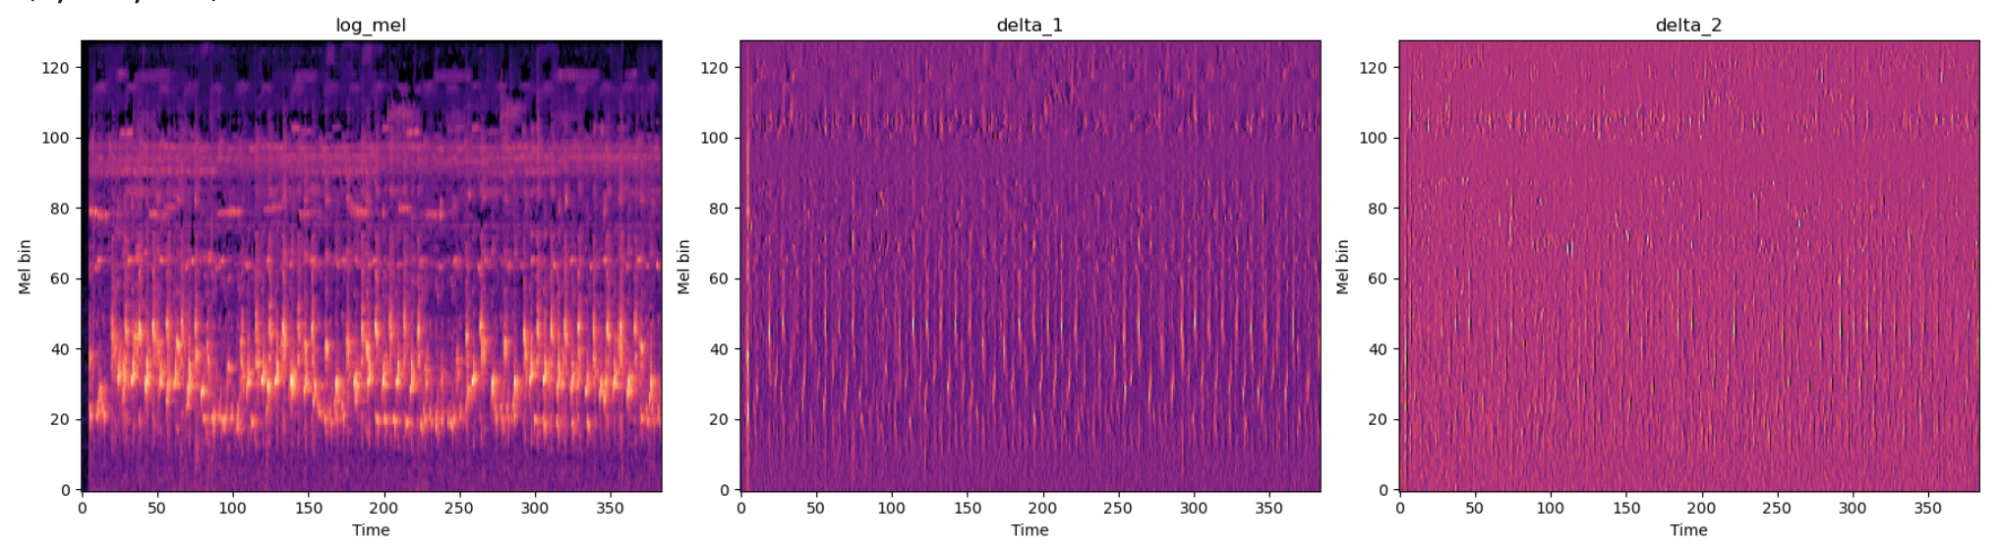
\includegraphics[width=\linewidth]{input_features.png}
\caption{Illustration of the three input channels: log-mel (left), first-order
delta (centre) and second-order delta (right). This example was rendered at
an earlier, coarser resolution (128 mel bins); the study uses 256 mel bins and
313 frames.}
\label{fig:input}
\end{figure}

\subsection{Student network}
\paragraph{Backbone.} An ImageNet-pretrained ResNet-18~\cite{he2016} truncated
after \texttt{layer4}, with the global average pool and fully connected layer
removed. For a $256\times313$ input it outputs a feature map
$H\in\mathbb{R}^{512\times8\times10}$ (channels $\times$ frequency $\times$
time). Each time step covers about 0.5\,s.

\paragraph{SED head (default, \var{HEAD=sed}).}
\begin{enumerate}
  \item \textbf{GeM frequency pooling} with a learnable exponent $p$
        (initialised at 3, clamped at $p\ge1$):
        $h_t=\big(\tfrac1F\sum_f H_{:,f,t}^{\,p}\big)^{1/p}$. With $p=1$ fixed
        this becomes mean pooling (\var{mean\_freq\_pool}).
  \item A bottleneck: Dropout(0.25) $\rightarrow$ Linear(512$\rightarrow$512)
        $\rightarrow$ ReLU $\rightarrow$ Dropout(0.5), applied at each time
        step.
  \item Two $1\times1$ temporal convolutions give attention logits $a_{c,t}$
        and frame logits $z_{c,t}$ for each class $c$:
        \begin{equation}
          \alpha_{c,t}=\frac{\exp(\tanh a_{c,t})}{\sum_{t'}\exp(\tanh a_{c,t'})},\qquad
          \hat y^{\text{clip}}_c=\sum_t\alpha_{c,t}\,z_{c,t},\qquad
          \hat y^{\text{fmax}}_c=\max_t z_{c,t}.
        \end{equation}
        \var{mean\_time\_pool} replaces $\alpha_{c,t}$ with $1/T$.
\end{enumerate}
At inference the window probability is the blend
$p_c=\tfrac12\sigma(\hat y^{\text{clip}}_c)+\tfrac12\sigma(\hat y^{\text{fmax}}_c)$.
The post-hoc variants \var{head\_clip\_only} and \var{head\_framemax\_only}
use one term each.

\paragraph{Pooled baseline (\var{HEAD=pooled}).} The plain ResNet-18:
frequency-averaged features, dropout(0.2) and a linear classifier per time
step, with clip logits taken as the mean over time. No distillation is used.

\paragraph{Distillation head.} A training-only branch,
GAP$(H)\rightarrow$Linear(512$\rightarrow$1536), regresses the cached Perch~v2
embedding $e^{\text{Perch}}$ of the same window~\cite{perch,hinton2015}:
\begin{equation}
  \mathcal L_{\text{dist}}=\frac1{1536}\big\|W\,\mathrm{GAP}(H)-e^{\text{Perch}}\big\|_2^2 .
\end{equation}
\textbf{Stop-gradient.} When distillation is on (default), the classification
head reads $\mathrm{stopgrad}(H)$. \emph{The backbone is therefore trained
only by the distillation loss}, and the classification loss updates only the
head. \var{distill\_no\_stopgrad} lets both losses update the backbone;
\var{no\_distill} removes the branch, so the backbone trains end-to-end on
classification. The branch is dropped at export, so distillation adds nothing
to inference cost.

\subsection{Perch pseudo-labels}
\label{sec:pseudo}
Perch~v2 is run once, offline and on the GPU, over every 5\,s window. It
supplies a 1536-d embedding (the distillation target), per-frame embeddings
($16\times1536$, for the probe baseline) and class logits. Perch classes are
mapped to competition classes by scientific name. Unmapped non-sonotype
species in Aves, Amphibia and Insecta use a \emph{genus proxy}: the maximum
over Perch classes of the same genus.

\paragraph{Focal windows (\var{USE\_PSEUDO\_FOCAL}).} A focal clip's labels
say \emph{which} species are present, and Perch says \emph{when}. For each
labelled species $c$ of a clip with windows $w$,
\begin{equation}
  \tilde y_{w,c}=\frac{p_c(w)}{\max_{w'}p_c(w')},
\end{equation}
and every other class is set to 0. If Perch cannot detect the species anywhere
in the clip ($\max_w p_c(w)<0.05$), every window keeps the hard label 1. The
ablation \var{no\_pseudo\_focal} uses the clip's hard primary + secondary
labels for every window.

\paragraph{Unlabelled soundscapes (\var{USE\_PSEUDO\_SC}).} Perch scores are
fused in logit space with a shrunk site/hour prior (described next). The
weights are $\lambda=0.4$ for mapped ``event'' taxa (birds), 1.0 for mapped
``texture'' taxa (frogs, insects) and 0.8 for texture genus proxies. Classes
with no Perch mapping receive the prior alone, and unmapped classes never seen
in labelled soundscapes are set to $-8$. Scores are then smoothed across the
12 windows of a file (neighbour averaging 0.35 for texture taxa, local-max
0.15 for event taxa) and passed through a sigmoid to give soft targets. The
prior tables for fold $k$ exclude fold-$k$ files.

\paragraph{Site/hour prior.} From labelled windows, species frequencies are
tabulated globally, per hour, per site and per (site, hour). They are shrunk
hierarchically as global $\rightarrow$ hour ($k=8$) $\rightarrow$ site ($k=8$)
$\rightarrow$ site-hour ($k=4$), with the weight of each level equal to
$n/(n+k)$, and converted to logits.

\subsection{Training}
\begin{itemize}
  \item \textbf{Data streams and batch composition.} Each batch of 64 is drawn
        with fixed shares: 70\% focal windows, 10\% labelled soundscape
        windows (other folds) and 20\% pseudo-labelled soundscape windows,
        renormalised when a stream is disabled. For fold 0 the streams hold
        121{,}805 focal, 624 labelled-soundscape and 24{,}000 pseudo windows;
        folds 1 and 2 are similar.
  \item \textbf{Rare upsampling.} Species with fewer than 20 focal windows are
        repeated up to 20. This affects 15 species and grows the focal
        windows from 152{,}198 to 152{,}431. \var{no\_rare\_upsample} sets
        the minimum to 0.
  \item \textbf{Mixup}~\cite{zhang2018}. Focal--focal mixup ($p=0.5$, $\lambda\sim
        \mathrm{Beta}(0.4,0.4)$) and focal--soundscape mixup with a labelled
        soundscape window from another fold ($p=0.5$,
        $\mathrm{Beta}(0.4,0.4)$). Mixing is done in the power domain,
        $10\log_{10}(\lambda10^{a/10}+(1-\lambda)10^{b/10})$, which is
        equivalent to mixing the audio. Labels are combined by union
        (``hard'' mixup), and Perch embeddings are mixed with the same
        $\lambda$.
  \item \textbf{SpecAugment}~\cite{park2019}: one frequency mask ($\le$10
        bins) and two time masks ($\le$10 frames).
  \item \textbf{Loss.} $\mathcal L=\mathcal L_{\text{cls}}+1.0\cdot\mathcal
        L_{\text{dist}}$, where $\mathcal L_{\text{cls}}=\tfrac12\mathrm{BCE}(\hat
        y^{\text{clip}},\tilde y)+\tfrac12\mathrm{BCE}(\hat y^{\text{fmax}},\tilde y)$,
        averaged over classes and weighted per source (focal, labelled
        soundscape and pseudo soundscape all 1.0).
  \item \textbf{Optimisation.} AdamW, constant learning rate $5\times10^{-4}$,
        weight decay $10^{-4}$, gradient clipping at norm 1.0, mixed
        precision, seed 42.
  \item \textbf{Budget.} 10 epochs of 600 batches (6{,}000 steps, about 2.6
        passes over the focal windows), cut from the notebook's 25 full epochs
        to make the ablations affordable.
  \item \textbf{Checkpoint selection.} After every epoch the model is scored
        on its validation fold, and the epoch with the best macro ROC-AUC over
        \emph{all} that fold's soundscape windows (S22 included) is kept.
\end{itemize}
The waveform gain and noise augmentation in the original notebook were
dropped when spectrograms were precomputed.

\subsection{Baselines}
\begin{description}
  \item[\var{resnet\_baseline}] Pooled ResNet-18 head, no distillation; all
        other settings as in \var{full}.
  \item[\var{perch\_attn\_probe}] Frozen Perch~v2 per-frame embeddings
        ($16\times1536$) $\rightarrow$ LayerNorm $\rightarrow$ the same
        attention-pooling head without the hidden layer. It uses the same
        training streams, targets and folds and is trained for 30 epochs
        (batch 256, AdamW, learning rate $10^{-3}$, weight decay $10^{-4}$).
        It answers how good the teacher alone is, and what running Perch on
        site would cost.
\end{description}

\subsection{Study design}
\label{sec:design}
Each training variant changes exactly one setting relative to \var{full}
(Table~\ref{tab:variants}). Post-hoc variants reuse \var{full}'s
out-of-fold predictions.

\begin{table}[H]
\centering\small
\caption{The 20 variants.}
\label{tab:variants}
\begin{tabular}{p{4cm}p{10.5cm}}
\toprule
Variant & Change relative to \var{full} \\
\midrule
\var{resnet\_baseline} & Pooled ResNet-18 head, no distillation \\
\var{perch\_attn\_probe} & Frozen Perch~v2 + attention-pooling linear probe (no CNN) \\
\var{full} & All components on \\
\midrule
\var{no\_distill} & No Perch distillation (backbone trained by classification) \\
\var{distill\_no\_stopgrad} & Distillation on, but classification gradients also reach the backbone \\
\var{no\_pseudo\_focal} & Hard clip labels on every focal window \\
\var{no\_pseudo\_sc} & No pseudo-labelled soundscape stream \\
\var{single\_channel\_mel} & Log-mel only (1 channel) \\
\var{mean\_freq\_pool} & Mean instead of GeM over frequency \\
\var{mean\_time\_pool} & Uniform instead of attention weights over time \\
\var{no\_mixup} & No focal--focal or focal--soundscape mixup \\
\var{no\_soundscape\_data} & No labelled soundscapes, no focal--soundscape mixup, no pseudo soundscapes \\
\var{no\_specaug} & No frequency/time masking \\
\var{no\_rare\_upsample} & No upsampling of species with $<$20 windows \\
\midrule
\var{head\_clip\_only} & Attention-pooled clip probability only \\
\var{head\_framemax\_only} & Frame-max probability only \\
\var{full+gauss\_smooth} & 5-tap kernel $(0.1,0.2,0.4,0.2,0.1)$ over neighbouring windows, in logit space \\
\var{full+tax\_smooth} & Pull each species toward its genus mean ($\alpha=0.15$), then class mean ($\alpha=0.05$) \\
\var{full+site\_hour\_prior} & Add fold-safe site/hour prior logits ($\lambda=1.0$ frogs/insects, 0.4 others) \\
\var{full+all\_posthoc} & Prior $\rightarrow$ Gaussian smoothing $\rightarrow$ taxonomy smoothing \\
\bottomrule
\end{tabular}
\end{table}

\subsection{Metrics}
All metrics are computed on the pooled out-of-fold predictions for the 192
evaluation windows (Section~\ref{sec:evalset}), ordered by file and time.
Classes without both a positive and a negative are skipped.
\begin{itemize}
  \item \textbf{Macro ROC-AUC} (primary): mean of per-class ROC-AUC.
  \item \textbf{Macro PR-AUC}: mean per-class average precision. The chance
        level equals class prevalence (0.069 on average here).
  \item \textbf{LRAP}: label-ranking average precision, i.e.\ how well the
        true species are ranked within each window.
  \item \textbf{Macro F1} at a threshold of 0.5.
  \item \textbf{ECE}: expected calibration error with 15 bins over all
        (window, class) cells. \textbf{Brier}: mean squared error of the
        probabilities.
  \item \textbf{Temporal jitter}: mean $|p_t-p_{t-1}|$ between consecutive
        windows of the same file.
  \item \textbf{AUC rare / common}: macro ROC-AUC over classes with $<$20 /
        $\ge$100 focal clips.
  \item \textbf{AUC per taxon}: macro ROC-AUC over Aves, Amphibia, Insecta and
        Mammalia classes. Reptilia has no scorable class here.
\end{itemize}

\subsection{Cost measurement and hardware}
Training ran on one NVIDIA L4 (GCP \texttt{g2-standard-16}) with three runs
sharing the GPU at a time, each with 4 data-loader workers. The offline Perch
pass took 830\,s of wall time (0.231 GPU-hours) for the 24{,}792 soundscape
windows. Inference cost (\texttt{benchmark\_cost.py}) rebuilds each network
from its \texttt{config.json} and times features + network on random input:
single-thread and 4-thread CPU at batch 12 (one 60\,s file), and GPU at batch
64. Perch is timed on the GPU only. The trained fold checkpoints were exported to ONNX and checked against
PyTorch. All 30 exports recorded in the logs agree to a maximum relative logit
difference of $2.2\times10^{-4}$.

% ===========================================================================
\section{Results}
\label{sec:results}

\subsection{Main results}
Tables~\ref{tab:main_rank} and~\ref{tab:main_calib} give every metric for
every variant. Figure~\ref{fig:aucbars} summarises the primary metric.

\begin{table}[H]\centering\small
\caption{Ranking and detection metrics for every variant on the pooled out-of-fold non-S22 soundscape windows (higher is better; best per column in bold).}\label{tab:main_rank}
\setlength{\tabcolsep}{3.5pt}
\begin{adjustbox}{max width=\linewidth}
\begin{tabular}{lrrrrrr}
\toprule
Variant & Macro ROC-AUC & Macro PR-AUC & LRAP & Macro F1 & AUC rare & AUC common \\
\midrule
\multicolumn{7}{l}{\emph{Baselines}} \\
\texttt{resnet\_baseline} & 0.7571 & 0.3618 & 0.2772 & \textbf{0.2522} & 0.7104 & 0.8387 \\
\texttt{perch\_attn\_probe} & 0.7109 & 0.3991 & 0.1390 & 0.1654 & 0.5778 & \textbf{0.9042} \\
\midrule
\multicolumn{7}{l}{\emph{Full model}} \\
\texttt{full} & 0.7142 & 0.3634 & 0.2209 & 0.1337 & 0.6679 & 0.7654 \\
\midrule
\multicolumn{7}{l}{\emph{One-change training ablations}} \\
\texttt{no\_distill} & 0.7292 & 0.3308 & 0.1820 & 0.1013 & 0.7004 & 0.7697 \\
\texttt{distill\_no\_stopgrad} & 0.6970 & 0.3738 & 0.2238 & 0.2349 & 0.6823 & 0.6460 \\
\texttt{no\_pseudo\_focal} & 0.7049 & 0.3675 & 0.1887 & 0.1261 & 0.6876 & 0.7004 \\
\texttt{no\_pseudo\_sc} & 0.7742 & \textbf{0.4321} & \textbf{0.4770} & 0.2396 & 0.7417 & 0.8174 \\
\texttt{single\_channel\_mel} & 0.7230 & 0.3744 & 0.1862 & 0.1446 & 0.6841 & 0.7714 \\
\texttt{mean\_freq\_pool} & 0.7466 & 0.4048 & 0.2897 & 0.2178 & 0.7165 & 0.7825 \\
\texttt{mean\_time\_pool} & 0.6984 & 0.3687 & 0.2101 & 0.1260 & 0.6651 & 0.7277 \\
\texttt{no\_mixup} & 0.6630 & 0.3396 & 0.1596 & 0.0866 & 0.6270 & 0.6813 \\
\texttt{no\_soundscape\_data} & 0.6656 & 0.1874 & 0.0589 & 0.0000 & 0.5822 & 0.8675 \\
\texttt{no\_specaug} & 0.7135 & 0.3607 & 0.2789 & 0.1692 & 0.6685 & 0.7538 \\
\texttt{no\_rare\_upsample} & 0.6896 & 0.3719 & 0.1956 & 0.1331 & 0.6636 & 0.6784 \\
\midrule
\multicolumn{7}{l}{\emph{Post-hoc variants of \texttt{full} (no retraining)}} \\
\texttt{head\_clip\_only} & 0.7050 & 0.3546 & 0.2267 & 0.0917 & 0.6703 & 0.7239 \\
\texttt{head\_framemax\_only} & 0.7145 & 0.3642 & 0.2141 & 0.1363 & 0.6620 & 0.7810 \\
\texttt{full+gauss\_smooth} & 0.7206 & 0.3940 & 0.2185 & 0.1221 & 0.6772 & 0.7622 \\
\texttt{full+tax\_smooth} & 0.7632 & 0.3743 & 0.2092 & 0.1046 & 0.7308 & 0.7631 \\
\texttt{full+site\_hour\_prior} & 0.7346 & 0.3608 & 0.3964 & 0.1575 & 0.6962 & 0.7432 \\
\texttt{full+all\_posthoc} & \textbf{0.8407} & 0.4159 & 0.4082 & 0.1164 & \textbf{0.8335} & 0.7987 \\
\bottomrule
\end{tabular}
\end{adjustbox}
\end{table}

\begin{table}[H]\centering\small
\caption{Calibration, temporal stability and per-taxon macro ROC-AUC for every variant (ECE, Brier and jitter: lower is better). Best per column in bold.}\label{tab:main_calib}
\setlength{\tabcolsep}{3.5pt}
\begin{adjustbox}{max width=\linewidth}
\begin{tabular}{lrrrrrrr}
\toprule
Variant & ECE$\downarrow$ & Brier$\downarrow$ & Jitter$\downarrow$ & AUC Aves & AUC Amph. & AUC Insecta & AUC Mamm. \\
\midrule
\multicolumn{8}{l}{\emph{Baselines}} \\
\texttt{resnet\_baseline} & 0.2256 & 0.1503 & 0.0684 & 0.8064 & 0.8347 & 0.6652 & 0.8245 \\
\texttt{perch\_attn\_probe} & 0.3564 & 0.2216 & 0.0860 & \textbf{0.8972} & 0.8625 & 0.4908 & 0.8185 \\
\midrule
\multicolumn{8}{l}{\emph{Full model}} \\
\texttt{full} & 0.1836 & 0.0931 & 0.0437 & 0.7509 & 0.8442 & 0.6401 & 0.4516 \\
\midrule
\multicolumn{8}{l}{\emph{One-change training ablations}} \\
\texttt{no\_distill} & 0.2249 & 0.1462 & 0.0620 & 0.7651 & 0.7791 & 0.7045 & 0.4322 \\
\texttt{distill\_no\_stopgrad} & 0.2501 & 0.1691 & 0.0519 & 0.6709 & 0.7802 & 0.6797 & 0.4890 \\
\texttt{no\_pseudo\_focal} & 0.2136 & 0.1152 & 0.0407 & 0.6849 & 0.8227 & 0.6512 & 0.6135 \\
\texttt{no\_pseudo\_sc} & \textbf{0.0032} & \textbf{0.0092} & 0.0027 & 0.8026 & 0.8961 & 0.6673 & \textbf{0.8447} \\
\texttt{single\_channel\_mel} & 0.2509 & 0.1467 & 0.0397 & 0.7572 & 0.8340 & 0.6382 & 0.6638 \\
\texttt{mean\_freq\_pool} & 0.1808 & 0.0931 & 0.0454 & 0.7709 & 0.8568 & 0.6548 & 0.7771 \\
\texttt{mean\_time\_pool} & 0.2183 & 0.1131 & 0.0391 & 0.7201 & 0.7993 & 0.6394 & 0.4956 \\
\texttt{no\_mixup} & 0.2377 & 0.1246 & 0.0494 & 0.6614 & 0.8192 & 0.6035 & 0.4272 \\
\texttt{no\_soundscape\_data} & 0.0078 & 0.0128 & 0.0016 & 0.8078 & 0.5871 & 0.6478 & 0.4066 \\
\texttt{no\_specaug} & 0.2180 & 0.1204 & 0.0403 & 0.7616 & 0.8277 & 0.6090 & 0.6939 \\
\texttt{no\_rare\_upsample} & 0.2281 & 0.1245 & 0.0441 & 0.7038 & 0.8163 & 0.6136 & 0.5735 \\
\midrule
\multicolumn{8}{l}{\emph{Post-hoc variants of \texttt{full} (no retraining)}} \\
\texttt{head\_clip\_only} & 0.1477 & 0.0733 & 0.0404 & 0.7171 & 0.8367 & 0.6430 & 0.4525 \\
\texttt{head\_framemax\_only} & 0.2196 & 0.1176 & 0.0505 & 0.7638 & 0.8457 & 0.6349 & 0.4364 \\
\texttt{full+gauss\_smooth} & 0.1814 & 0.0902 & 0.0124 & 0.7468 & 0.8573 & 0.6485 & 0.4668 \\
\texttt{full+tax\_smooth} & 0.1836 & 0.0917 & 0.0434 & 0.7450 & \textbf{0.9173} & 0.7217 & 0.4287 \\
\texttt{full+site\_hour\_prior} & 0.0059 & 0.0102 & 0.0045 & 0.7591 & 0.8383 & 0.6599 & 0.6240 \\
\texttt{full+all\_posthoc} & 0.0062 & 0.0100 & \textbf{0.0013} & 0.7943 & 0.9139 & \textbf{0.8558} & 0.5662 \\
\bottomrule
\end{tabular}
\end{adjustbox}
\end{table}


\begin{figure}[H]
\centering
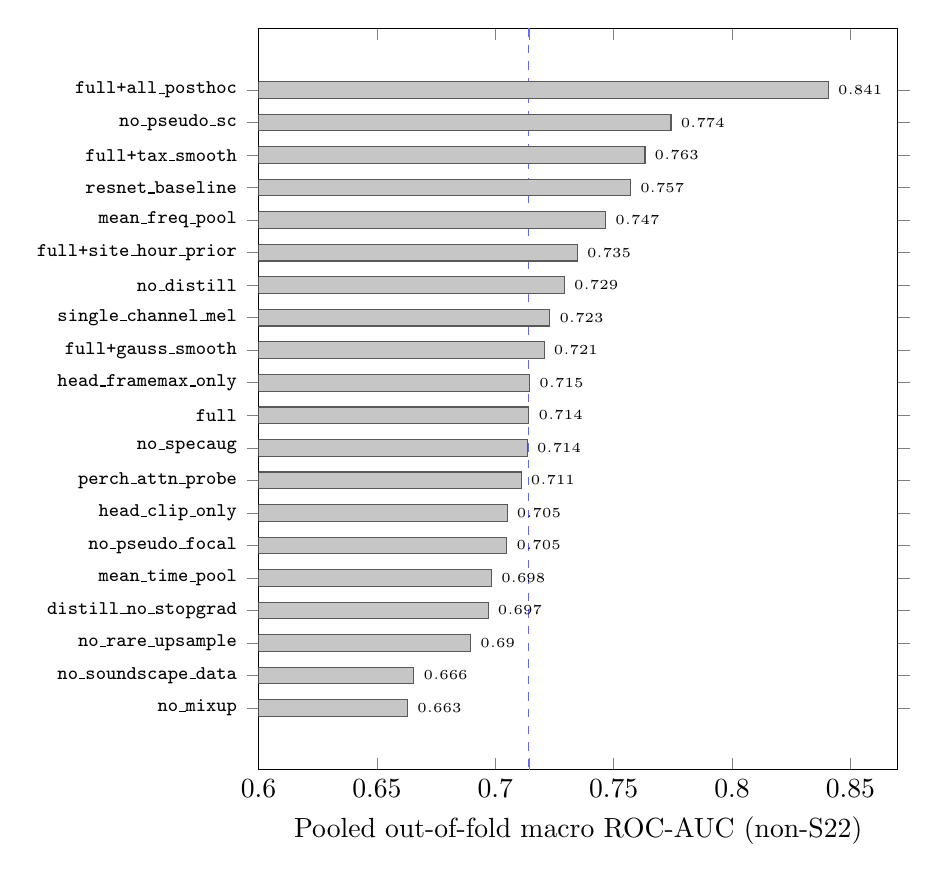
\begin{tikzpicture}
\begin{axis}[xbar, bar width=6pt, width=0.8\linewidth, height=11cm,
  xmin=0.6, xmax=0.87, xlabel={Pooled out-of-fold macro ROC-AUC (non-S22)},
  symbolic y coords={full+all\_posthoc,no\_pseudo\_sc,full+tax\_smooth,resnet\_baseline,mean\_freq\_pool,full+site\_hour\_prior,no\_distill,single\_channel\_mel,full+gauss\_smooth,head\_framemax\_only,full,no\_specaug,perch\_attn\_probe,head\_clip\_only,no\_pseudo\_focal,mean\_time\_pool,distill\_no\_stopgrad,no\_rare\_upsample,no\_soundscape\_data,no\_mixup},
  ytick=data, y dir=reverse, yticklabel style={font=\scriptsize\ttfamily},
  nodes near coords, nodes near coords style={font=\tiny,/pgf/number format/.cd,fixed,precision=3},
  extra x ticks={0.7142}, extra x tick labels={}, extra x tick style={grid=major, grid style={dashed,blue!60}}]
\addplot[fill=gray!45, draw=gray!70!black] coordinates {
 (0.8407,full+all\_posthoc) (0.7742,no\_pseudo\_sc) (0.7632,full+tax\_smooth) (0.7571,resnet\_baseline)
 (0.7466,mean\_freq\_pool) (0.7346,full+site\_hour\_prior) (0.7292,no\_distill) (0.7230,single\_channel\_mel)
 (0.7206,full+gauss\_smooth) (0.7145,head\_framemax\_only) (0.7142,full) (0.7135,no\_specaug)
 (0.7109,perch\_attn\_probe) (0.7050,head\_clip\_only) (0.7049,no\_pseudo\_focal) (0.6984,mean\_time\_pool)
 (0.6970,distill\_no\_stopgrad) (0.6896,no\_rare\_upsample) (0.6656,no\_soundscape\_data) (0.6630,no\_mixup)};
\end{axis}
\end{tikzpicture}
\caption{All 20 variants ranked by the primary metric. The dashed line marks
\var{full} (0.7142).}
\label{fig:aucbars}
\end{figure}

The headline results are:
\begin{itemize}
  \item \textbf{Best overall:} \var{full+all\_posthoc} has a macro ROC-AUC of
        0.8407, rare-class AUC 0.8335, Insecta 0.8558, ECE 0.0062 and jitter
        0.0013, at the inference cost of \var{full}.
  \item \textbf{Best trained model:} \var{no\_pseudo\_sc} leads on macro AUC
        (0.7742), PR-AUC (0.4321), LRAP (0.4770), ECE (0.0032), Brier
        (0.0092) and Mammalia AUC (0.8447).
  \item \textbf{The plain baseline beats the full model:}
        \var{resnet\_baseline} reaches 0.7571 (+0.0429 over \var{full}) and
        has the best macro F1 (0.2522).
  \item \textbf{The teacher alone} (\var{perch\_attn\_probe}) is best on
        common species (0.9042) and birds (0.8972), but worst on rare species
        (0.5778), insects (0.4908), ECE (0.3564), Brier (0.2216) and jitter
        (0.0860), and second-worst on LRAP (0.1390).
  \item \textbf{The two most damaging removals} are mixup (0.6630) and
        soundscape data (0.6656). The latter predicts nothing above 0.5
        (F1 = 0.0000) and has PR-AUC 0.1874, but has the second-highest
        common-species AUC (0.8675).
\end{itemize}

\subsection{Changes relative to the full model}
Tables~\ref{tab:delta_rank} and~\ref{tab:delta_calib} give the change from
\var{full} for every metric.

\begin{table}[H]\centering\small
\caption{Change relative to \texttt{full} (variant $-$ full) for the ranking metrics.}\label{tab:delta_rank}
\setlength{\tabcolsep}{3.5pt}
\begin{adjustbox}{max width=\linewidth}
\begin{tabular}{lrrrrrr}
\toprule
Variant & $\Delta$AUC & $\Delta$PR-AUC & $\Delta$LRAP & $\Delta$F1 & $\Delta$rare & $\Delta$common \\
\midrule
\multicolumn{7}{l}{\emph{Baselines}} \\
\texttt{resnet\_baseline} & +0.0429 & $-$0.0016 & +0.0563 & +0.1185 & +0.0425 & +0.0733 \\
\texttt{perch\_attn\_probe} & $-$0.0032 & +0.0356 & $-$0.0820 & +0.0317 & $-$0.0901 & +0.1388 \\
\midrule
\multicolumn{7}{l}{\emph{One-change training ablations}} \\
\texttt{no\_distill} & +0.0150 & $-$0.0327 & $-$0.0389 & $-$0.0323 & +0.0325 & +0.0044 \\
\texttt{distill\_no\_stopgrad} & $-$0.0172 & +0.0103 & +0.0028 & +0.1013 & +0.0144 & $-$0.1194 \\
\texttt{no\_pseudo\_focal} & $-$0.0093 & +0.0040 & $-$0.0323 & $-$0.0076 & +0.0196 & $-$0.0650 \\
\texttt{no\_pseudo\_sc} & +0.0600 & +0.0686 & +0.2560 & +0.1059 & +0.0738 & +0.0521 \\
\texttt{single\_channel\_mel} & +0.0088 & +0.0110 & $-$0.0347 & +0.0109 & +0.0162 & +0.0060 \\
\texttt{mean\_freq\_pool} & +0.0325 & +0.0414 & +0.0688 & +0.0841 & +0.0486 & +0.0171 \\
\texttt{mean\_time\_pool} & $-$0.0158 & +0.0053 & $-$0.0108 & $-$0.0077 & $-$0.0028 & $-$0.0377 \\
\texttt{no\_mixup} & $-$0.0512 & $-$0.0239 & $-$0.0614 & $-$0.0471 & $-$0.0409 & $-$0.0841 \\
\texttt{no\_soundscape\_data} & $-$0.0486 & $-$0.1760 & $-$0.1620 & $-$0.1337 & $-$0.0857 & +0.1021 \\
\texttt{no\_specaug} & $-$0.0007 & $-$0.0027 & +0.0579 & +0.0355 & +0.0006 & $-$0.0116 \\
\texttt{no\_rare\_upsample} & $-$0.0245 & +0.0085 & $-$0.0254 & $-$0.0006 & $-$0.0043 & $-$0.0870 \\
\midrule
\multicolumn{7}{l}{\emph{Post-hoc variants of \texttt{full} (no retraining)}} \\
\texttt{head\_clip\_only} & $-$0.0092 & $-$0.0089 & +0.0058 & $-$0.0420 & +0.0024 & $-$0.0415 \\
\texttt{head\_framemax\_only} & +0.0003 & +0.0008 & $-$0.0068 & +0.0026 & $-$0.0059 & +0.0157 \\
\texttt{full+gauss\_smooth} & +0.0064 & +0.0306 & $-$0.0024 & $-$0.0116 & +0.0093 & $-$0.0032 \\
\texttt{full+tax\_smooth} & +0.0490 & +0.0108 & $-$0.0117 & $-$0.0291 & +0.0629 & $-$0.0023 \\
\texttt{full+site\_hour\_prior} & +0.0204 & $-$0.0027 & +0.1754 & +0.0238 & +0.0282 & $-$0.0221 \\
\texttt{full+all\_posthoc} & +0.1266 & +0.0524 & +0.1873 & $-$0.0173 & +0.1656 & +0.0333 \\
\bottomrule
\end{tabular}
\end{adjustbox}
\end{table}

\begin{table}[H]\centering\small
\caption{Change relative to \texttt{full} for calibration, jitter and per-taxon AUC (for ECE, Brier and jitter a negative change is an improvement).}\label{tab:delta_calib}
\setlength{\tabcolsep}{3.5pt}
\begin{adjustbox}{max width=\linewidth}
\begin{tabular}{lrrrrrrr}
\toprule
Variant & $\Delta$ECE & $\Delta$Brier & $\Delta$Jitter & $\Delta$Aves & $\Delta$Amph. & $\Delta$Insecta & $\Delta$Mamm. \\
\midrule
\multicolumn{8}{l}{\emph{Baselines}} \\
\texttt{resnet\_baseline} & +0.0419 & +0.0573 & +0.0247 & +0.0556 & $-$0.0095 & +0.0251 & +0.3729 \\
\texttt{perch\_attn\_probe} & +0.1727 & +0.1285 & +0.0423 & +0.1463 & +0.0183 & $-$0.1493 & +0.3670 \\
\midrule
\multicolumn{8}{l}{\emph{One-change training ablations}} \\
\texttt{no\_distill} & +0.0413 & +0.0531 & +0.0183 & +0.0142 & $-$0.0651 & +0.0643 & $-$0.0194 \\
\texttt{distill\_no\_stopgrad} & +0.0665 & +0.0760 & +0.0082 & $-$0.0800 & $-$0.0640 & +0.0396 & +0.0374 \\
\texttt{no\_pseudo\_focal} & +0.0299 & +0.0221 & $-$0.0030 & $-$0.0660 & $-$0.0215 & +0.0111 & +0.1619 \\
\texttt{no\_pseudo\_sc} & $-$0.1804 & $-$0.0839 & $-$0.0411 & +0.0517 & +0.0519 & +0.0272 & +0.3931 \\
\texttt{single\_channel\_mel} & +0.0673 & +0.0536 & $-$0.0040 & +0.0063 & $-$0.0102 & $-$0.0019 & +0.2122 \\
\texttt{mean\_freq\_pool} & $-$0.0028 & $-$0.0000 & +0.0017 & +0.0201 & +0.0126 & +0.0147 & +0.3255 \\
\texttt{mean\_time\_pool} & +0.0347 & +0.0200 & $-$0.0046 & $-$0.0308 & $-$0.0450 & $-$0.0007 & +0.0440 \\
\texttt{no\_mixup} & +0.0540 & +0.0315 & +0.0057 & $-$0.0894 & $-$0.0250 & $-$0.0366 & $-$0.0244 \\
\texttt{no\_soundscape\_data} & $-$0.1759 & $-$0.0803 & $-$0.0421 & +0.0569 & $-$0.2571 & +0.0077 & $-$0.0450 \\
\texttt{no\_specaug} & +0.0343 & +0.0273 & $-$0.0034 & +0.0108 & $-$0.0165 & $-$0.0312 & +0.2423 \\
\texttt{no\_rare\_upsample} & +0.0445 & +0.0314 & +0.0004 & $-$0.0470 & $-$0.0279 & $-$0.0265 & +0.1219 \\
\midrule
\multicolumn{8}{l}{\emph{Post-hoc variants of \texttt{full} (no retraining)}} \\
\texttt{head\_clip\_only} & $-$0.0360 & $-$0.0198 & $-$0.0033 & $-$0.0338 & $-$0.0075 & +0.0029 & +0.0009 \\
\texttt{head\_framemax\_only} & +0.0360 & +0.0245 & +0.0068 & +0.0129 & +0.0015 & $-$0.0052 & $-$0.0152 \\
\texttt{full+gauss\_smooth} & $-$0.0023 & $-$0.0029 & $-$0.0313 & $-$0.0041 & +0.0130 & +0.0084 & +0.0152 \\
\texttt{full+tax\_smooth} & $-$0.0000 & $-$0.0014 & $-$0.0003 & $-$0.0059 & +0.0731 & +0.0816 & $-$0.0229 \\
\texttt{full+site\_hour\_prior} & $-$0.1777 & $-$0.0829 & $-$0.0392 & +0.0082 & $-$0.0059 & +0.0198 & +0.1724 \\
\texttt{full+all\_posthoc} & $-$0.1774 & $-$0.0831 & $-$0.0424 & +0.0435 & +0.0697 & +0.2157 & +0.1146 \\
\bottomrule
\end{tabular}
\end{adjustbox}
\end{table}


\subsection{Statistical uncertainty}
\label{sec:boot}
The evaluation set has only 16 files, and windows within a file are strongly
correlated. We therefore ran a \emph{file-level} bootstrap: the 16 files were
resampled with replacement 2{,}000 times (seed 0), and macro ROC-AUC was
recomputed for every trained variant on each resample. Paired differences
against \var{full} use the same resamples. The post-hoc variants need the
competition taxonomy file, which is not stored with the results, so they are
not bootstrapped.

\begin{table}[H]\centering\small
\caption{File-level bootstrap (2{,}000 resamples of the 16 evaluation files) of pooled macro ROC-AUC. The 95\% interval is the 2.5--97.5 percentile range. $\Delta$ is the paired difference to \texttt{full} on the same resamples; $P(\Delta>0)$ is the fraction of resamples in which the variant beats \texttt{full}. Intervals whose $\Delta$ range excludes 0 are marked $\ast$.}
\label{tab:boot}
\begin{adjustbox}{max width=\linewidth}
\begin{tabular}{lrcrcr}
\toprule
Variant & Macro AUC & 95\% CI & $\Delta$ vs full & 95\% CI of $\Delta$ & $P(\Delta>0)$ \\
\midrule
\texttt{no\_pseudo\_sc} & 0.7742 & [0.703, 0.872] & +0.0600 & [$-$0.0009, +0.1513] & 0.974 \\
\texttt{resnet\_baseline} & 0.7571 & [0.665, 0.858] & +0.0429 & [$-$0.0114, +0.1098] & 0.943 \\
\texttt{mean\_freq\_pool} & 0.7466 & [0.662, 0.849] & +0.0325 & [+0.0018, +0.0735]$\ast$ & 0.979 \\
\texttt{no\_distill} & 0.7292 & [0.632, 0.824] & +0.0150 & [$-$0.0408, +0.0794] & 0.675 \\
\texttt{single\_channel\_mel} & 0.7230 & [0.637, 0.826] & +0.0088 & [$-$0.0281, +0.0527] & 0.690 \\
\texttt{full} & 0.7142 & [0.622, 0.820] & -- & -- & -- \\
\texttt{no\_specaug} & 0.7135 & [0.626, 0.808] & $-$0.0007 & [$-$0.0413, +0.0456] & 0.468 \\
\texttt{perch\_attn\_probe} & 0.7109 & [0.622, 0.798] & $-$0.0032 & [$-$0.0945, +0.0737] & 0.408 \\
\texttt{no\_pseudo\_focal} & 0.7049 & [0.604, 0.814] & $-$0.0093 & [$-$0.0481, +0.0281] & 0.274 \\
\texttt{mean\_time\_pool} & 0.6984 & [0.606, 0.811] & $-$0.0158 & [$-$0.0414, +0.0196] & 0.230 \\
\texttt{distill\_no\_stopgrad} & 0.6970 & [0.580, 0.798] & $-$0.0172 & [$-$0.0886, +0.0389] & 0.249 \\
\texttt{no\_rare\_upsample} & 0.6896 & [0.600, 0.793] & $-$0.0245 & [$-$0.0573, +0.0213] & 0.133 \\
\texttt{no\_soundscape\_data} & 0.6656 & [0.582, 0.723] & $-$0.0486 & [$-$0.1919, +0.0503] & 0.151 \\
\texttt{no\_mixup} & 0.6630 & [0.559, 0.764] & $-$0.0512 & [$-$0.1113, $-$0.0144]$\ast$ & 0.006 \\
\bottomrule
\end{tabular}
\end{adjustbox}
\end{table}


The intervals are wide. \var{full}'s macro AUC has a 95\% interval of
[0.622, 0.820], about $\pm0.10$. Only two paired differences exclude zero:
\var{mean\_freq\_pool} is better than \var{full} (+0.0325, interval
[+0.002, +0.074], better in 97.9\% of resamples) and \var{no\_mixup} is worse
($-0.0512$, interval [$-0.111$, $-0.014$], better in only 0.6\% of
resamples). \var{no\_pseudo\_sc} (+0.0600, better in 97.4\% of resamples,
interval [$-0.001$, +0.151]) and \var{resnet\_baseline} (+0.0429, 94.3\%)
are borderline. Every other difference in macro AUC, including
\var{no\_soundscape\_data} ($-0.0486$, interval [$-0.192$, +0.050]), is
within resampling noise for this metric.

\subsection{Pooled versus fold-local scores}
\label{sec:pooled}
Each fold's checkpoint is chosen on that fold's validation windows
(Table~\ref{tab:perfold}). Scored \emph{within} a fold, the non-S22 macro AUC
of the selected checkpoints is 0.70--0.94 (0.54 for \var{no\_soundscape\_data}
on fold 1). For \var{full} the mean of the three folds is 0.825. The pooled out-of-fold scores in
Table~\ref{tab:main_rank} are much lower (0.66--0.77). Table~\ref{tab:foldlocal}
gives the fold-local macro AUC on the evaluation windows.

\begingroup\footnotesize
\begin{table}[H]\centering
\caption{Per-fold checkpoint selection for the CNN variants (\texttt{history.json}). The saved checkpoint is the epoch with the best macro ROC-AUC over \emph{all} validation windows of that fold (S22 included); ``non-S22 @best'' is the fold-local non-S22 macro AUC of that checkpoint and ``max non-S22'' the best value reached in any epoch. Fold-local numbers are higher than the pooled out-of-fold score (Section~\ref{sec:pooled}).}
\label{tab:perfold}
\setlength{\tabcolsep}{3pt}
\begin{adjustbox}{max width=\linewidth}
\begin{tabular}{lrrrrrrrrr}
\toprule
 & \multicolumn{3}{c}{Fold 0} & \multicolumn{3}{c}{Fold 1} & \multicolumn{3}{c}{Fold 2} \\
\cmidrule(lr){2-4}\cmidrule(lr){5-7}\cmidrule(lr){8-10}
Variant & best ep & non-S22 @best & max non-S22 & best ep & non-S22 @best & max non-S22 & best ep & non-S22 @best & max non-S22 \\
\midrule
\texttt{resnet\_baseline} & 3 & 0.8808 & 0.8808 & 9 & 0.8606 & 0.9073 & 9 & 0.8781 & 0.8781 \\
\texttt{full} & 5 & 0.8177 & 0.8214 & 9 & 0.8385 & 0.8499 & 6 & 0.8196 & 0.8476 \\
\texttt{no\_distill} & 2 & 0.8233 & 0.8491 & 7 & 0.8950 & 0.8950 & 5 & 0.8461 & 0.8461 \\
\texttt{distill\_no\_stopgrad} & 9 & 0.7228 & 0.8030 & 6 & 0.8508 & 0.8545 & 9 & 0.7943 & 0.7943 \\
\texttt{no\_pseudo\_focal} & 5 & 0.8004 & 0.8004 & 8 & 0.8645 & 0.8645 & 8 & 0.8483 & 0.8483 \\
\texttt{no\_pseudo\_sc} & 9 & 0.9228 & 0.9228 & 6 & 0.8955 & 0.8976 & 9 & 0.9412 & 0.9412 \\
\texttt{single\_channel\_mel} & 8 & 0.8852 & 0.8959 & 8 & 0.8802 & 0.8862 & 8 & 0.8475 & 0.8696 \\
\texttt{mean\_freq\_pool} & 9 & 0.8838 & 0.8838 & 9 & 0.8780 & 0.8955 & 9 & 0.8777 & 0.8844 \\
\texttt{mean\_time\_pool} & 8 & 0.8021 & 0.8315 & 9 & 0.8564 & 0.8790 & 9 & 0.8780 & 0.8780 \\
\texttt{no\_mixup} & 8 & 0.7384 & 0.7557 & 8 & 0.8210 & 0.8210 & 9 & 0.7998 & 0.7998 \\
\texttt{no\_soundscape\_data} & 9 & 0.7436 & 0.7436 & 1 & 0.5387 & 0.6713 & 9 & 0.7241 & 0.7241 \\
\texttt{no\_specaug} & 8 & 0.8016 & 0.8016 & 9 & 0.8852 & 0.8852 & 8 & 0.8582 & 0.8748 \\
\texttt{no\_rare\_upsample} & 8 & 0.7902 & 0.7902 & 7 & 0.8816 & 0.8816 & 9 & 0.8567 & 0.8567 \\
\bottomrule
\end{tabular}
\end{adjustbox}
\end{table}
\endgroup

\begin{table}[H]\centering\small
\caption{Fold-local macro ROC-AUC: each fold's selected checkpoint scored only on that fold's non-S22 evaluation windows, versus the pooled out-of-fold score over all 192 windows.}
\label{tab:foldlocal}
\begin{tabular}{lrrrrr}
\toprule
Variant & Fold 0 & Fold 1 & Fold 2 & Mean of folds & Pooled \\
\midrule
\texttt{no\_pseudo\_sc} & 0.9228 & 0.8955 & 0.9412 & 0.9198 & 0.7742 \\
\texttt{resnet\_baseline} & 0.8808 & 0.8606 & 0.8781 & 0.8732 & 0.7571 \\
\texttt{mean\_freq\_pool} & 0.8838 & 0.8780 & 0.8777 & 0.8799 & 0.7466 \\
\texttt{no\_distill} & 0.8233 & 0.8950 & 0.8461 & 0.8548 & 0.7292 \\
\texttt{single\_channel\_mel} & 0.8852 & 0.8802 & 0.8475 & 0.8710 & 0.7230 \\
\texttt{full} & 0.8177 & 0.8385 & 0.8196 & 0.8253 & 0.7142 \\
\texttt{no\_specaug} & 0.8016 & 0.8852 & 0.8582 & 0.8483 & 0.7135 \\
\texttt{perch\_attn\_probe} & 0.7495 & 0.7015 & 0.8207 & 0.7572 & 0.7109 \\
\texttt{no\_pseudo\_focal} & 0.8004 & 0.8645 & 0.8483 & 0.8378 & 0.7049 \\
\texttt{mean\_time\_pool} & 0.8021 & 0.8564 & 0.8780 & 0.8455 & 0.6984 \\
\texttt{distill\_no\_stopgrad} & 0.7228 & 0.8508 & 0.7943 & 0.7893 & 0.6970 \\
\texttt{no\_rare\_upsample} & 0.7902 & 0.8816 & 0.8567 & 0.8428 & 0.6896 \\
\texttt{no\_soundscape\_data} & 0.7436 & 0.5387 & 0.7241 & 0.6688 & 0.6656 \\
\texttt{no\_mixup} & 0.7384 & 0.8210 & 0.7998 & 0.7864 & 0.6630 \\
\bottomrule
\end{tabular}
\end{table}


\subsection{Pre-registered hypotheses}
Before training, each variant was given the metric it should move most and
the expected direction (Table~\ref{tab:hyp}). \textbf{13 of 21} hypotheses
were supported.

\begingroup\footnotesize
\begin{longtable}{p{3.1cm}p{3.3cm}p{1.4cm}rp{2.9cm}p{1.8cm}}
\caption{Pre-registered hypotheses (one per row, from \texttt{configs.py}) against the observed change relative to \texttt{full}. ``Biggest-$\Delta$'' is the metric that moved most in absolute terms. The rationale written before the runs is given in italics.}\label{tab:hyp}\\
\toprule Variant & Metric & Predicted & $\Delta$ vs full & Biggest-$\Delta$ & Verdict \\ \midrule
\endfirsthead
\toprule Variant & Metric & Predicted & $\Delta$ vs full & Biggest-$\Delta$ & Verdict \\ \midrule
\endhead
\bottomrule
\endlastfoot
\texttt{resnet\_baseline} & \texttt{lrap} & drop & +0.0563 & \texttt{auc\_Mammalia} & not supported \\
\multicolumn{6}{p{15cm}}{\emph{A plain pooled ResNet loses the time axis, so it ranks species within a window worse (LRAP) and is less calibrated than the attention SED head at the same cost.}} \\[2pt]
\texttt{resnet\_baseline} & \texttt{ece} & rise & +0.0419 & \texttt{auc\_Mammalia} & \textbf{supported} \\
\multicolumn{6}{p{15cm}}{\emph{Without distillation or frame-level heads the baseline overfits the small label set.}} \\[2pt]
\texttt{perch\_attn\_probe} & \texttt{auc\_rare} & rise & $-$0.0901 & \texttt{auc\_Mammalia} & not supported \\
\multicolumn{6}{p{15cm}}{\emph{Perch has seen far more data; the frozen teacher should beat the student on rare species, at many times the inference cost (see benchmark\_cost.py).}} \\[2pt]
\texttt{no\_pseudo\_focal} & \texttt{pr\_auc\_macro} & drop & +0.0040 & \texttt{auc\_Mammalia} & not supported \\
\multicolumn{6}{p{15cm}}{\emph{Clip-level labels mark every 5 s window as positive even when the bird is silent; Perch-localised targets remove those false positives, mainly helping precision (PR-AUC).}} \\[2pt]
\texttt{no\_pseudo\_sc} & \texttt{auc\_soundscape\_macro} & drop & +0.0600 & \texttt{auc\_Mammalia} & not supported \\
\multicolumn{6}{p{15cm}}{\emph{Unlabelled soundscapes are in-domain; their pseudo-labels should help soundscape AUC and calibration most.}} \\[2pt]
\texttt{single\_channel\_mel} & \texttt{auc\_Insecta} & drop & $-$0.0019 & \texttt{auc\_Mammalia} & \textbf{supported} \\
\multicolumn{6}{p{15cm}}{\emph{Delta channels encode modulation / onsets; insects and frogs are defined by repetition rate, so dropping them should hurt non-bird taxa more.}} \\[2pt]
\texttt{no\_distill} & \texttt{auc\_rare} & drop & +0.0325 & \texttt{auc\_Amphibia} & not supported \\
\multicolumn{6}{p{15cm}}{\emph{Perch embeddings carry knowledge about species with few focal clips.}} \\[2pt]
\texttt{no\_distill} & \texttt{ece} & rise & +0.0413 & \texttt{auc\_Amphibia} & \textbf{supported} \\
\multicolumn{6}{p{15cm}}{\emph{Without the teacher regulariser the student overfits, giving worse calibration.}} \\[2pt]
\texttt{distill\_no\_stopgrad} & \texttt{auc\_soundscape\_macro} & ~same & $-$0.0172 & \texttt{auc\_common} & not supported \\
\multicolumn{6}{p{15cm}}{\emph{Letting the classification loss update the backbone should matter little.}} \\[2pt]
\texttt{mean\_freq\_pool} & \texttt{auc\_Insecta} & drop & +0.0147 & \texttt{auc\_Mammalia} & not supported \\
\multicolumn{6}{p{15cm}}{\emph{GeM sharpens toward narrow bands; insects/frogs are narrow-band.}} \\[2pt]
\texttt{mean\_time\_pool} & \texttt{lrap} & drop & $-$0.0108 & \texttt{auc\_Amphibia} & \textbf{supported} \\
\multicolumn{6}{p{15cm}}{\emph{Attention pooling picks the frames with the call; uniform pooling dilutes short calls.}} \\[2pt]
\texttt{no\_soundscape\_data} & \texttt{auc\_soundscape\_macro} & drop & $-$0.0486 & \texttt{auc\_Amphibia} & \textbf{supported} \\
\multicolumn{6}{p{15cm}}{\emph{Soundscape windows match the deployment domain.}} \\[2pt]
\texttt{no\_mixup} & \texttt{f1\_macro} & drop & $-$0.0471 & \texttt{auc\_Aves} & \textbf{supported} \\
\multicolumn{6}{p{15cm}}{\emph{Mixup teaches multi-species windows, so multi-label F1 should drop more than AUC.}} \\[2pt]
\texttt{no\_specaug} & \texttt{auc\_soundscape\_macro} & small drop & $-$0.0007 & \texttt{auc\_Mammalia} & \textbf{supported} \\
\multicolumn{6}{p{15cm}}{\emph{SpecAugment is a generic regulariser; expect a small uniform drop.}} \\[2pt]
\texttt{no\_rare\_upsample} & \texttt{auc\_rare} & drop & $-$0.0043 & \texttt{auc\_Mammalia} & \textbf{supported} \\
\multicolumn{6}{p{15cm}}{\emph{Upsampling only touches species with <20 clips.}} \\[2pt]
\texttt{head\_clip\_only} & \texttt{lrap} & drop & +0.0058 & \texttt{f1\_macro} & not supported \\
\multicolumn{6}{p{15cm}}{\emph{Clip and frame-max heads make different errors; the 50/50 blend should beat either.}} \\[2pt]
\texttt{head\_framemax\_only} & \texttt{ece} & rise & +0.0360 & \texttt{ece} & \textbf{supported} \\
\multicolumn{6}{p{15cm}}{\emph{Max over frames is biased upward, so frame-max-only should be over-confident.}} \\[2pt]
\texttt{full+gauss\_smooth} & \texttt{temporal\_jitter} & drop & $-$0.0313 & \texttt{temporal\_jitter} & \textbf{supported} \\
\multicolumn{6}{p{15cm}}{\emph{Smoothing across neighbouring windows mainly reduces prediction jitter.}} \\[2pt]
\texttt{full+tax\_smooth} & \texttt{auc\_rare} & rise & +0.0629 & \texttt{auc\_Insecta} & \textbf{supported} \\
\multicolumn{6}{p{15cm}}{\emph{Rare species borrow evidence from relatives in the same genus.}} \\[2pt]
\texttt{full+site\_hour\_prior} & \texttt{auc\_soundscape\_macro} & rise & +0.0204 & \texttt{ece} & \textbf{supported} \\
\multicolumn{6}{p{15cm}}{\emph{Where and when a recording was made is a strong, free signal for which species can be present -- expected to be the best gain per unit of inference cost.}} \\[2pt]
\texttt{full+all\_posthoc} & \texttt{auc\_soundscape\_macro} & rise & +0.1266 & \texttt{auc\_Insecta} & \textbf{supported} \\
\multicolumn{6}{p{15cm}}{\emph{The free post-processing steps stack.}} \\[2pt]
\end{longtable}
\endgroup


\subsection{Inference and training cost}
\begin{table}[H]\centering\small
\caption{Measured inference cost per 5\,s window (\texttt{benchmark\_cost.py}). CPU timings use a batch of 12 windows (one 60\,s file) with 1 or 4 threads and include feature extraction (``feat''); GPU timings use a batch of 64 on the NVIDIA L4. Real-time factor = 5000\,ms / CPU-1 ms. Perch is GPU-only; for \texttt{perch\_attn\_probe} the parameter count and size are the probe head only, while the GPU time includes running Perch v2.}
\label{tab:cost}
\setlength{\tabcolsep}{3pt}
\begin{adjustbox}{max width=\linewidth}
\begin{tabular}{lrrrrrrrrr}
\toprule
Variant & Params (M) & Size (MB) & GFLOPs & CPU1 feat & CPU1 ms & CPU4 ms & GPU ms & GPU preds/s & RT$\times$ \\
\midrule
\texttt{resnet\_baseline} & 11.297 & 45.2 & 5.898 & 9.19 & 83.63 & 21.86 & 0.782 & 1279 & 59.8 \\
\texttt{perch\_attn\_probe} & 0.722 & 2.9 & -- & -- & -- & -- & 2.569 & 389 & -- \\
\texttt{full} & 11.679 & 46.7 & 5.906 & 9.02 & 81.92 & 22.02 & 0.785 & 1273 & 61.0 \\
\texttt{no\_distill} & 11.679 & 46.7 & 5.906 & 8.85 & 81.54 & 21.25 & 0.783 & 1276 & 61.3 \\
\texttt{distill\_no\_stopgrad} & 11.679 & 46.7 & 5.906 & 9.67 & 82.39 & 21.75 & 0.785 & 1275 & 60.7 \\
\texttt{no\_pseudo\_focal} & 11.679 & 46.7 & 5.906 & 9.28 & 82.03 & 22.89 & 0.784 & 1275 & 61.0 \\
\texttt{no\_pseudo\_sc} & 11.679 & 46.7 & 5.906 & 9.17 & 81.99 & 21.35 & 0.784 & 1275 & 61.0 \\
\texttt{single\_channel\_mel} & 11.673 & 46.7 & 5.654 & 8.12 & 80.82 & 22.57 & 0.731 & 1369 & 61.9 \\
\texttt{mean\_freq\_pool} & 11.679 & 46.7 & 5.906 & 9.02 & 81.39 & 22.02 & 0.783 & 1277 & 61.4 \\
\texttt{mean\_time\_pool} & 11.679 & 46.7 & 5.906 & 9.05 & 82.20 & 21.94 & 0.786 & 1273 & 60.8 \\
\texttt{no\_mixup} & 11.679 & 46.7 & 5.906 & 8.97 & 81.55 & 21.34 & 0.784 & 1275 & 61.3 \\
\texttt{no\_soundscape\_data} & 11.679 & 46.7 & 5.906 & 9.05 & 81.39 & 21.94 & 0.784 & 1275 & 61.4 \\
\texttt{no\_specaug} & 11.679 & 46.7 & 5.906 & 9.51 & 82.38 & 21.39 & 0.783 & 1277 & 60.7 \\
\texttt{no\_rare\_upsample} & 11.679 & 46.7 & 5.906 & 8.82 & 81.29 & 21.40 & 0.785 & 1274 & 61.5 \\
\bottomrule
\end{tabular}
\end{adjustbox}
\end{table}


All 12 ResNet-18 variants cost essentially the same: 11.68\,M parameters
(11.30\,M for the pooled baseline, 11.67\,M single-channel), 46.7\,MB, 5.91
GFLOPs (5.65 single-channel), 80.8--83.6\,ms per window on one CPU thread
(59.8--61.9$\times$ real time), 21.3--22.9\,ms with 4 threads, and
0.73--0.79\,ms on the GPU (about 1{,}270--1{,}370 windows/s). Feature
extraction is 8.1--9.7\,ms of the single-thread time. Running Perch~v2 with
the probe takes 2.57\,ms per window on the GPU (389 windows/s, 3.3$\times$ the
ResNet GPU time) and has no CPU path.

\begin{table}[H]\centering\small
\caption{Quality versus cost (\texttt{bang\_for\_buck.csv}), sorted by single-thread CPU time. Post-hoc variants inherit the cost of \texttt{full}. ``Gain/ms'' is the macro-AUC change relative to \texttt{resnet\_baseline} divided by the extra CPU milliseconds (undefined for the baseline itself and for the GPU-only probe). A variant is on the Pareto frontier if no other variant is both cheaper and better on macro ROC-AUC.}
\label{tab:bang}
\setlength{\tabcolsep}{3.5pt}
\begin{adjustbox}{max width=\linewidth}
\begin{tabular}{lrrrrrcc}
\toprule
Variant & Macro AUC & CPU1 ms & GPU ms & Train GPU-h & Gain/ms & Pareto (CPU) & Pareto (GPU) \\
\midrule
\texttt{single\_channel\_mel} & 0.7230 & 80.82 & 0.731 & 0.438 & +0.0121 & \checkmark & \checkmark \\
\texttt{no\_rare\_upsample} & 0.6896 & 81.29 & 0.785 & 0.315 & +0.0288 &  &  \\
\texttt{no\_soundscape\_data} & 0.6656 & 81.39 & 0.784 & 0.484 & +0.0407 &  &  \\
\texttt{mean\_freq\_pool} & 0.7466 & 81.39 & 0.783 & 0.477 & +0.0047 & \checkmark &  \\
\texttt{no\_distill} & 0.7292 & 81.54 & 0.783 & 0.485 & +0.0134 &  &  \\
\texttt{no\_mixup} & 0.6630 & 81.55 & 0.784 & 0.320 & +0.0452 &  &  \\
\texttt{full} & 0.7142 & 81.92 & 0.785 & 0.463 & +0.0250 &  &  \\
\texttt{head\_clip\_only} & 0.7050 & 81.92 & 0.785 & 0.463 & +0.0304 &  &  \\
\texttt{full+tax\_smooth} & 0.7632 & 81.92 & 0.785 & 0.463 & $-$0.0035 &  &  \\
\texttt{full+all\_posthoc} & 0.8407 & 81.92 & 0.785 & 0.463 & $-$0.0487 & \checkmark & \checkmark \\
\texttt{full+site\_hour\_prior} & 0.7346 & 81.92 & 0.785 & 0.463 & +0.0131 &  &  \\
\texttt{full+gauss\_smooth} & 0.7206 & 81.92 & 0.785 & 0.463 & +0.0213 &  &  \\
\texttt{head\_framemax\_only} & 0.7145 & 81.92 & 0.785 & 0.463 & +0.0248 &  &  \\
\texttt{no\_pseudo\_sc} & 0.7742 & 81.99 & 0.784 & 0.487 & $-$0.0104 &  & \checkmark \\
\texttt{no\_pseudo\_focal} & 0.7049 & 82.03 & 0.784 & 0.478 & +0.0325 &  &  \\
\texttt{mean\_time\_pool} & 0.6984 & 82.20 & 0.786 & 0.475 & +0.0411 &  &  \\
\texttt{no\_specaug} & 0.7135 & 82.38 & 0.783 & 0.328 & +0.0346 &  &  \\
\texttt{distill\_no\_stopgrad} & 0.6970 & 82.39 & 0.785 & 0.320 & +0.0484 &  &  \\
\texttt{resnet\_baseline} & 0.7571 & 83.63 & 0.782 & 0.458 & -- &  & \checkmark \\
\texttt{perch\_attn\_probe} & 0.7109 & -- & 2.569 & 0.156 & -- &  &  \\
\bottomrule
\end{tabular}
\end{adjustbox}
\end{table}


\begin{figure}[H]
\centering
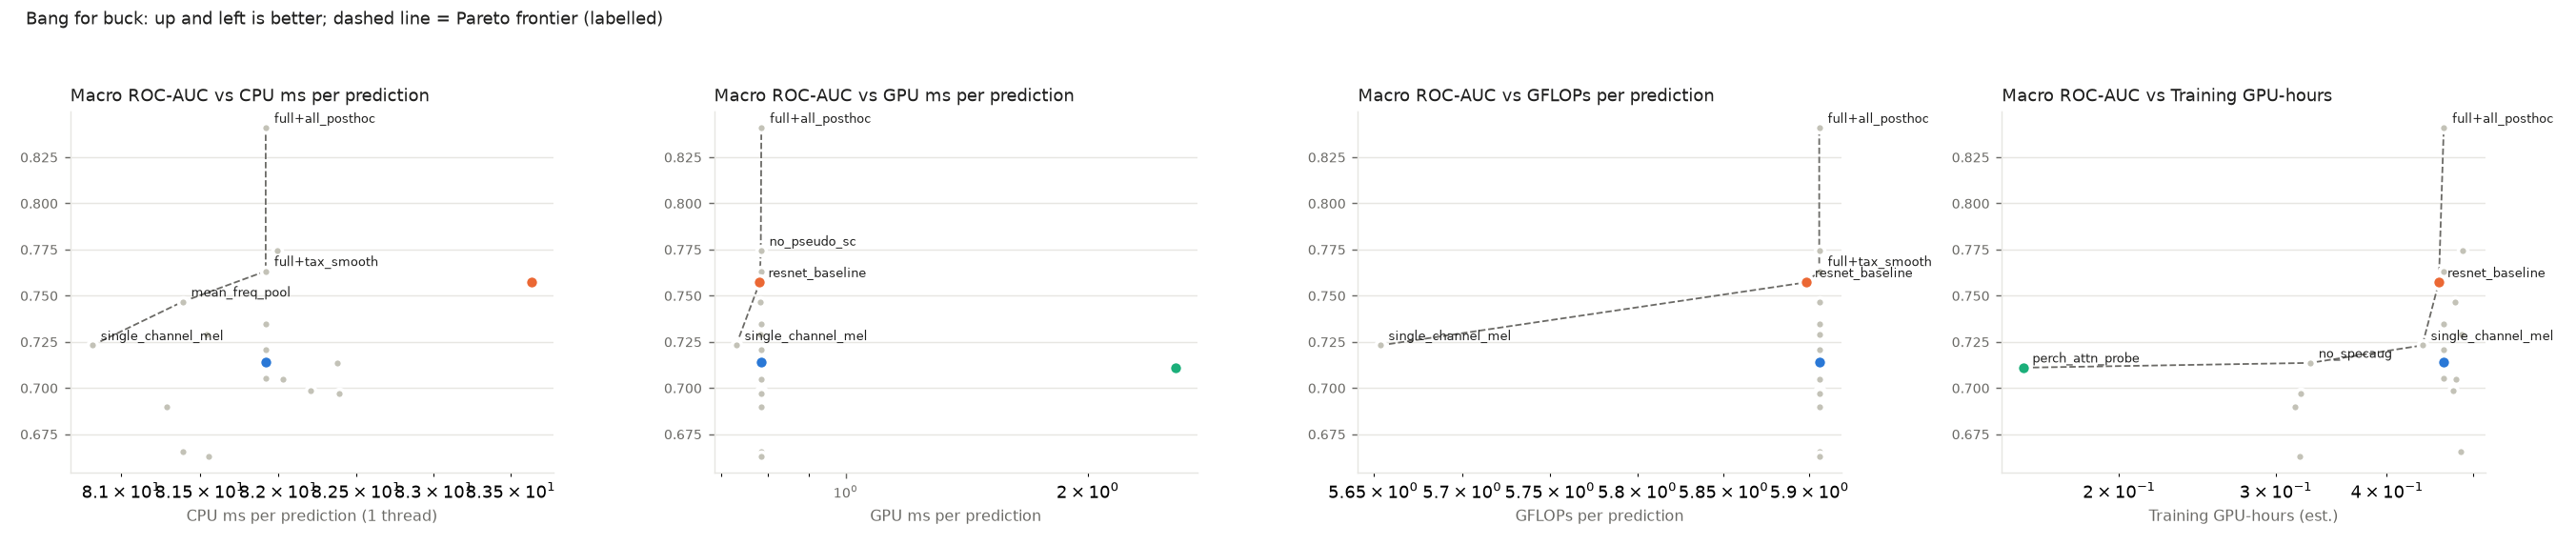
\includegraphics[width=\linewidth]{cost_vs_quality.png}
\caption{Quality against cost (CPU ms, GPU ms, GFLOPs and training GPU-hours
per prediction). Dashed lines are the Pareto frontiers. On CPU the frontier is
\var{single\_channel\_mel} $\rightarrow$ \var{mean\_freq\_pool} $\rightarrow$
\var{full+all\_posthoc}. On GPU it is \var{single\_channel\_mel} $\rightarrow$
\var{resnet\_baseline} $\rightarrow$ \var{no\_pseudo\_sc} $\rightarrow$
\var{full+all\_posthoc}.}
\label{fig:cost}
\end{figure}

\begin{table}[H]\centering\small
\caption{Training cost per variant (3 folds). Three runs shared one L4 GPU at a time, so GPU-hours are estimated as wall time / 3, and epoch times depend on what the other two lanes were running.}
\label{tab:traincost}
\begin{adjustbox}{max width=\linewidth}
\begin{tabular}{lrrrrr}
\toprule
Variant & Wall (s) & GPU-h (est.) & Mean epoch (s) & Peak GPU mem (GB) & Epochs \\
\midrule
\texttt{resnet\_baseline} & 4942 & 0.458 & 163.9 & 2.187 & 10 \\
\texttt{perch\_attn\_probe} & 1689 & 0.156 & -- & 0.143 & 30 \\
\texttt{full} & 5005 & 0.463 & 166.0 & 2.199 & 10 \\
\texttt{no\_distill} & 5241 & 0.485 & 173.9 & 2.190 & 10 \\
\texttt{distill\_no\_stopgrad} & 3455 & 0.320 & 114.4 & 2.196 & 10 \\
\texttt{no\_pseudo\_focal} & 5165 & 0.478 & 171.3 & 2.199 & 10 \\
\texttt{no\_pseudo\_sc} & 5262 & 0.487 & 174.5 & 2.196 & 10 \\
\texttt{single\_channel\_mel} & 4735 & 0.438 & 157.0 & 2.133 & 10 \\
\texttt{mean\_freq\_pool} & 5147 & 0.477 & 170.7 & 2.197 & 10 \\
\texttt{mean\_time\_pool} & 5129 & 0.475 & 170.1 & 2.198 & 10 \\
\texttt{no\_mixup} & 3451 & 0.320 & 114.3 & 2.199 & 10 \\
\texttt{no\_soundscape\_data} & 5224 & 0.484 & 173.3 & 2.199 & 10 \\
\texttt{no\_specaug} & 3541 & 0.328 & 117.3 & 2.199 & 10 \\
\texttt{no\_rare\_upsample} & 3405 & 0.315 & 112.8 & 2.199 & 10 \\
\bottomrule
\end{tabular}
\end{adjustbox}
\end{table}


\subsection{Training dynamics}
\begin{table}[H]\centering\scriptsize
\caption{Pooled out-of-fold non-S22 macro ROC-AUC after every epoch (\texttt{all\_curves.csv}). For the Perch probe (30 epochs) the first 10 epochs and the final epoch are shown. Best epoch per row in bold.}
\label{tab:curve}
\setlength{\tabcolsep}{2.5pt}
\begin{adjustbox}{max width=\linewidth}
\begin{tabular}{lrrrrrrrrrrr}
\toprule
Variant & ep0 & ep1 & ep2 & ep3 & ep4 & ep5 & ep6 & ep7 & ep8 & ep9 & ep29 \\
\midrule
\texttt{resnet\_baseline} & 0.648 & 0.710 & 0.725 & 0.743 & 0.725 & 0.726 & 0.731 & 0.711 & 0.718 & \textbf{0.761} & -- \\
\texttt{perch\_attn\_probe} & 0.679 & 0.693 & 0.703 & 0.705 & 0.703 & 0.705 & 0.715 & 0.703 & 0.711 & 0.711 & 0.711 \\
\texttt{full} & 0.512 & 0.452 & 0.495 & 0.552 & 0.634 & 0.662 & 0.690 & 0.677 & 0.697 & \textbf{0.713} & -- \\
\texttt{no\_distill} & 0.562 & 0.617 & 0.684 & 0.690 & 0.678 & 0.715 & 0.717 & 0.709 & \textbf{0.732} & 0.680 & -- \\
\texttt{distill\_no\_stopgrad} & 0.465 & 0.640 & 0.673 & 0.680 & 0.655 & 0.692 & 0.696 & 0.664 & 0.686 & \textbf{0.709} & -- \\
\texttt{no\_pseudo\_focal} & 0.519 & 0.448 & 0.500 & 0.519 & 0.600 & 0.655 & 0.682 & 0.679 & 0.698 & \textbf{0.707} & -- \\
\texttt{no\_pseudo\_sc} & 0.463 & 0.517 & 0.618 & 0.694 & 0.715 & 0.723 & 0.749 & 0.760 & 0.755 & \textbf{0.764} & -- \\
\texttt{single\_channel\_mel} & 0.459 & 0.434 & 0.476 & 0.566 & 0.643 & 0.674 & 0.704 & 0.712 & \textbf{0.723} & 0.719 & -- \\
\texttt{mean\_freq\_pool} & 0.492 & 0.487 & 0.521 & 0.552 & 0.620 & 0.647 & 0.696 & 0.705 & 0.722 & \textbf{0.747} & -- \\
\texttt{mean\_time\_pool} & 0.498 & 0.462 & 0.482 & 0.494 & 0.572 & 0.608 & 0.646 & 0.669 & 0.686 & \textbf{0.706} & -- \\
\texttt{no\_mixup} & 0.512 & 0.449 & 0.468 & 0.452 & 0.516 & 0.555 & 0.597 & 0.606 & 0.639 & \textbf{0.677} & -- \\
\texttt{no\_soundscape\_data} & 0.455 & 0.495 & 0.558 & 0.559 & 0.552 & 0.611 & 0.606 & 0.652 & 0.673 & \textbf{0.704} & -- \\
\texttt{no\_specaug} & 0.494 & 0.531 & 0.507 & 0.599 & 0.640 & 0.682 & 0.679 & 0.702 & \textbf{0.710} & 0.710 & -- \\
\texttt{no\_rare\_upsample} & 0.500 & 0.441 & 0.491 & 0.505 & 0.587 & 0.616 & 0.647 & 0.666 & 0.681 & \textbf{0.701} & -- \\
\bottomrule
\end{tabular}
\end{adjustbox}
\end{table}


\begin{figure}[H]
\centering
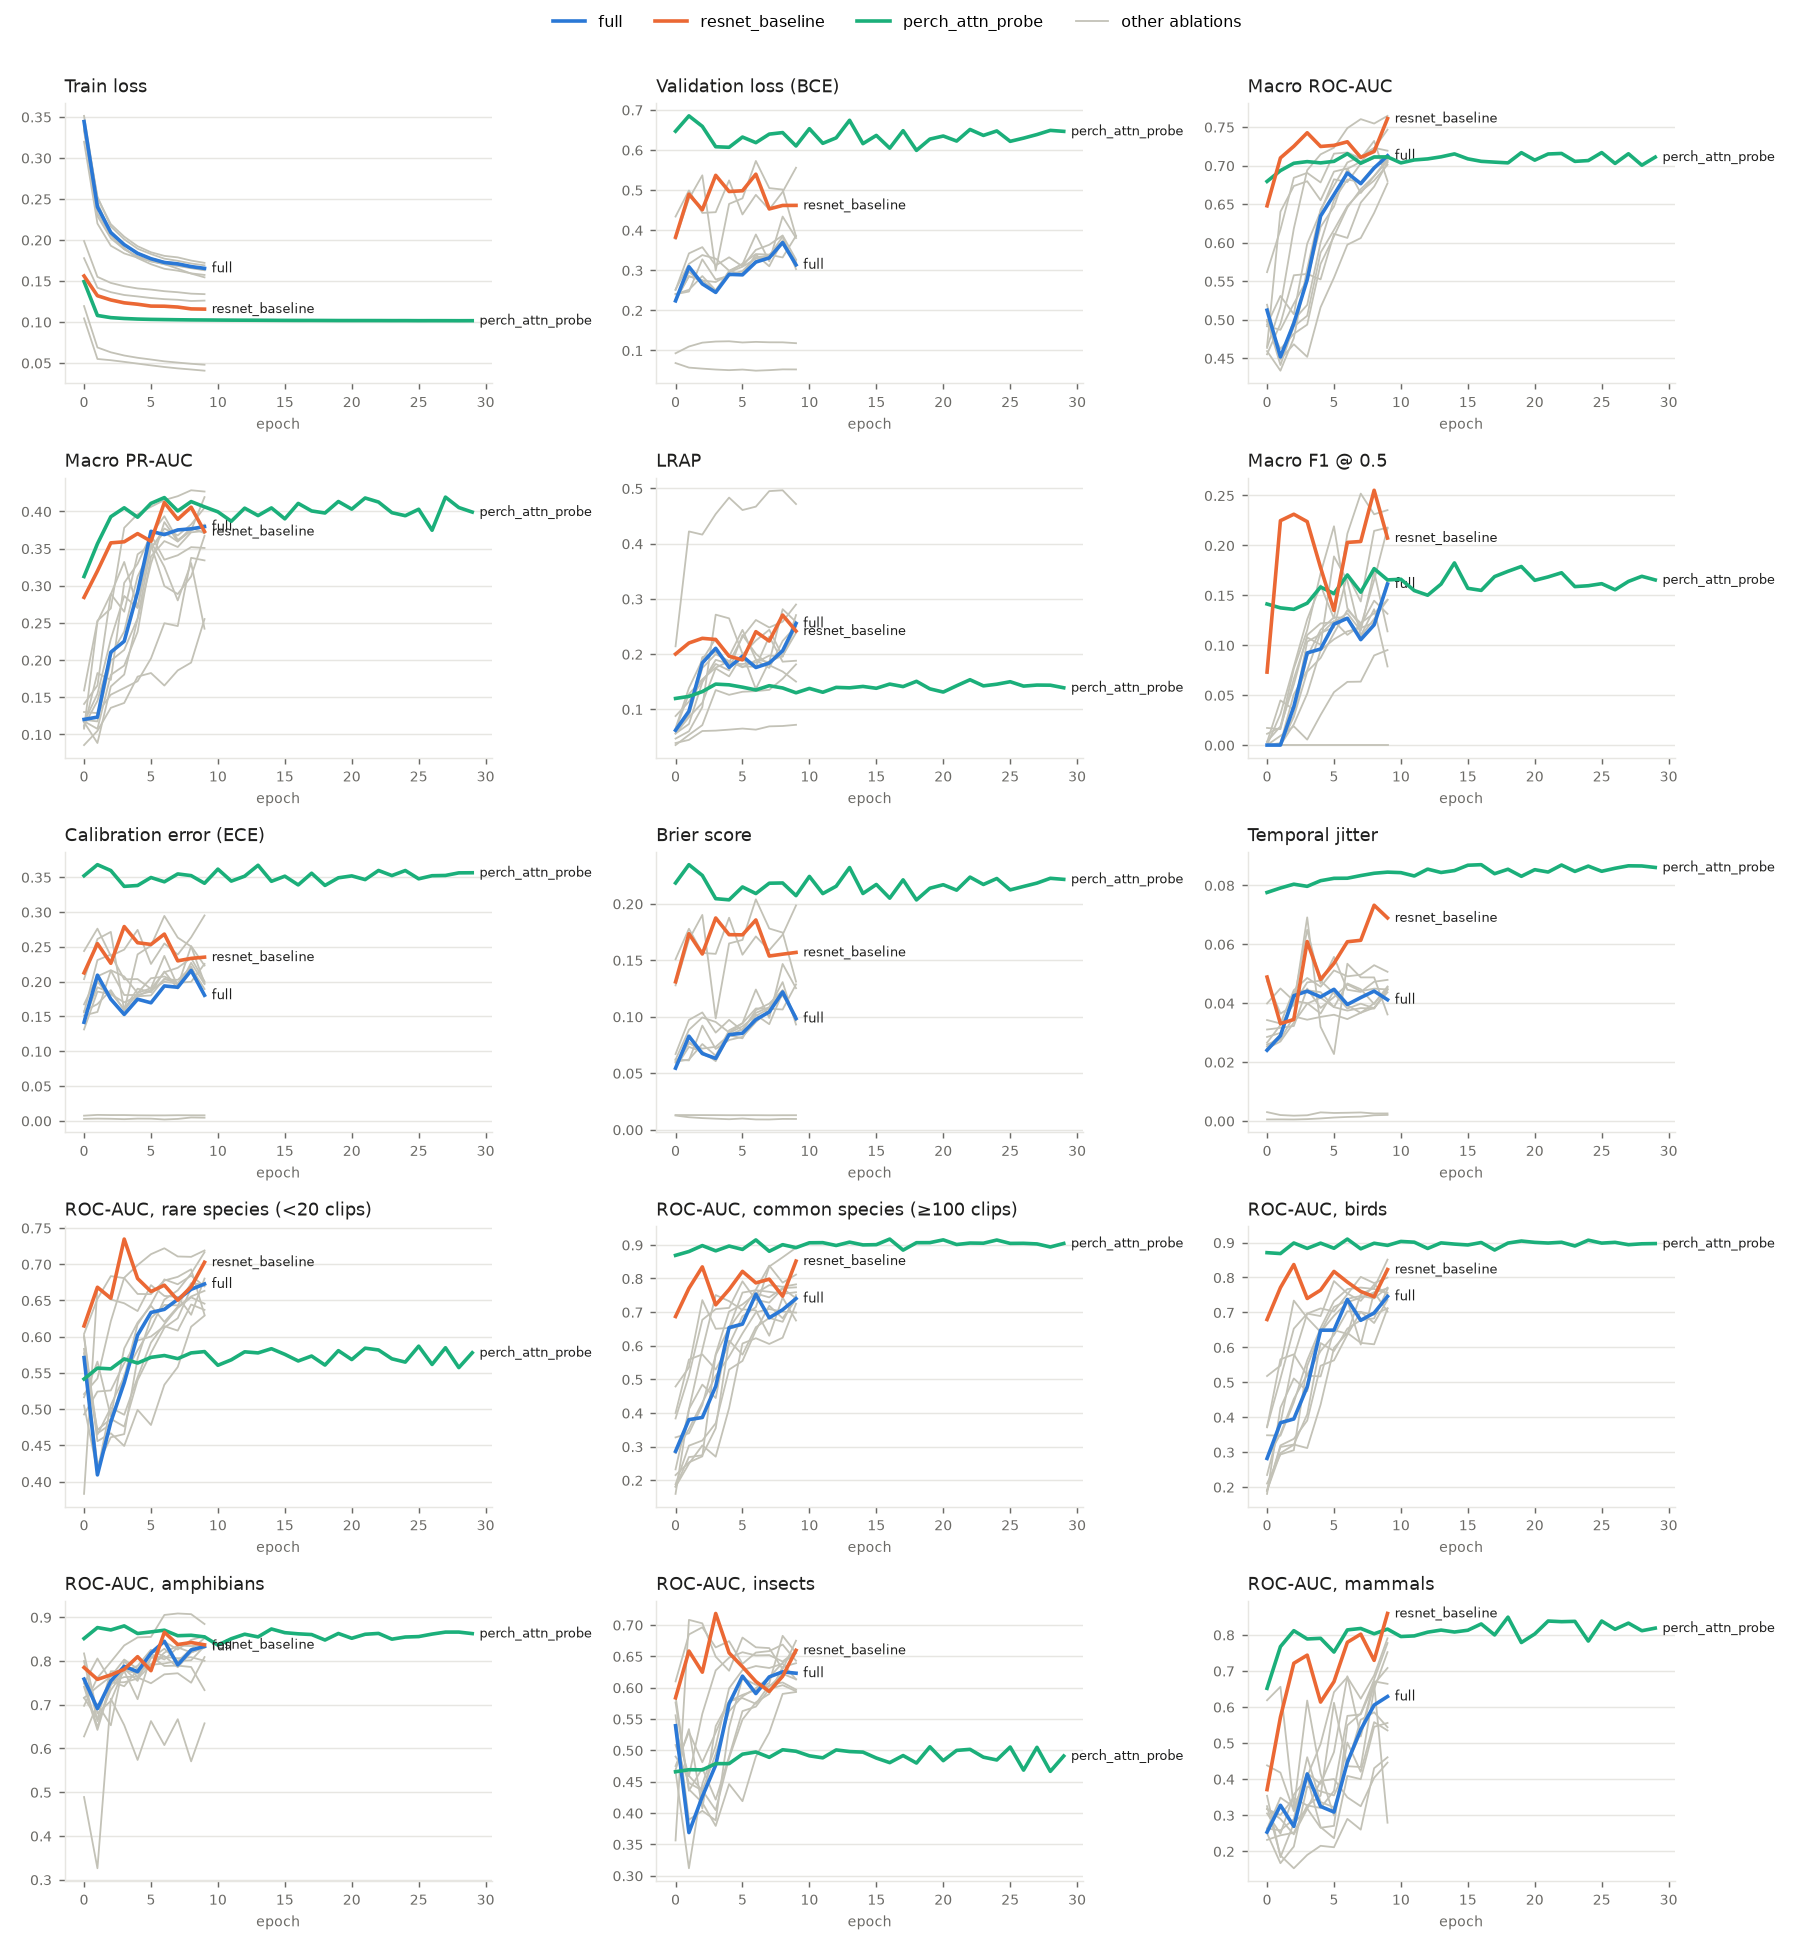
\includegraphics[width=\linewidth]{learning_curves.png}
\caption{Pooled learning curves for all metrics. \var{full} (blue),
\var{resnet\_baseline} (orange) and \var{perch\_attn\_probe} (green) are
highlighted; grey lines are the other ablations.}
\label{fig:curves}
\end{figure}

Four patterns stand out (Table~\ref{tab:curve}, Figure~\ref{fig:curves}):
\begin{enumerate}
  \item \textbf{Slow start of the distilled models.} \var{full}'s pooled AUC
        is 0.512, 0.452 and 0.495 in epochs 0--2, below or near chance, and
        then rises steadily to 0.713 at epoch 9. It is \emph{still rising at
        the end of the budget}. The same shape appears for every variant
        with stop-gradient distillation.
  \item \textbf{Fast start without stop-gradient.} \var{resnet\_baseline}
        reaches 0.710 after two epochs (epoch 1) and ends at 0.761.
        \var{no\_distill} reaches 0.684 by epoch 2, peaks at 0.732 (epoch 8)
        and falls to 0.680 at epoch 9. \var{distill\_no\_stopgrad} reaches
        0.640 at epoch 1.
  \item \textbf{Perch probe plateau.} The probe is at 0.679 after one epoch
        and then fluctuates between 0.693 and 0.717 for 29 more epochs.
  \item \textbf{Calibration drift.} \var{full}'s validation BCE rises from
        0.22 to 0.31--0.37 while AUC improves, and its ECE stays around
        0.15--0.22. The variants without pseudo-labelled soundscapes
        (\var{no\_pseudo\_sc}, \var{no\_soundscape\_data}) keep validation
        BCE near 0.05--0.12 and ECE below 0.01 throughout. Training loss
        follows the same split: 0.35$\rightarrow$0.17 for \var{full} versus
        0.12$\rightarrow$0.05 for \var{no\_pseudo\_sc}.
\end{enumerate}

\begin{figure}[H]
\centering
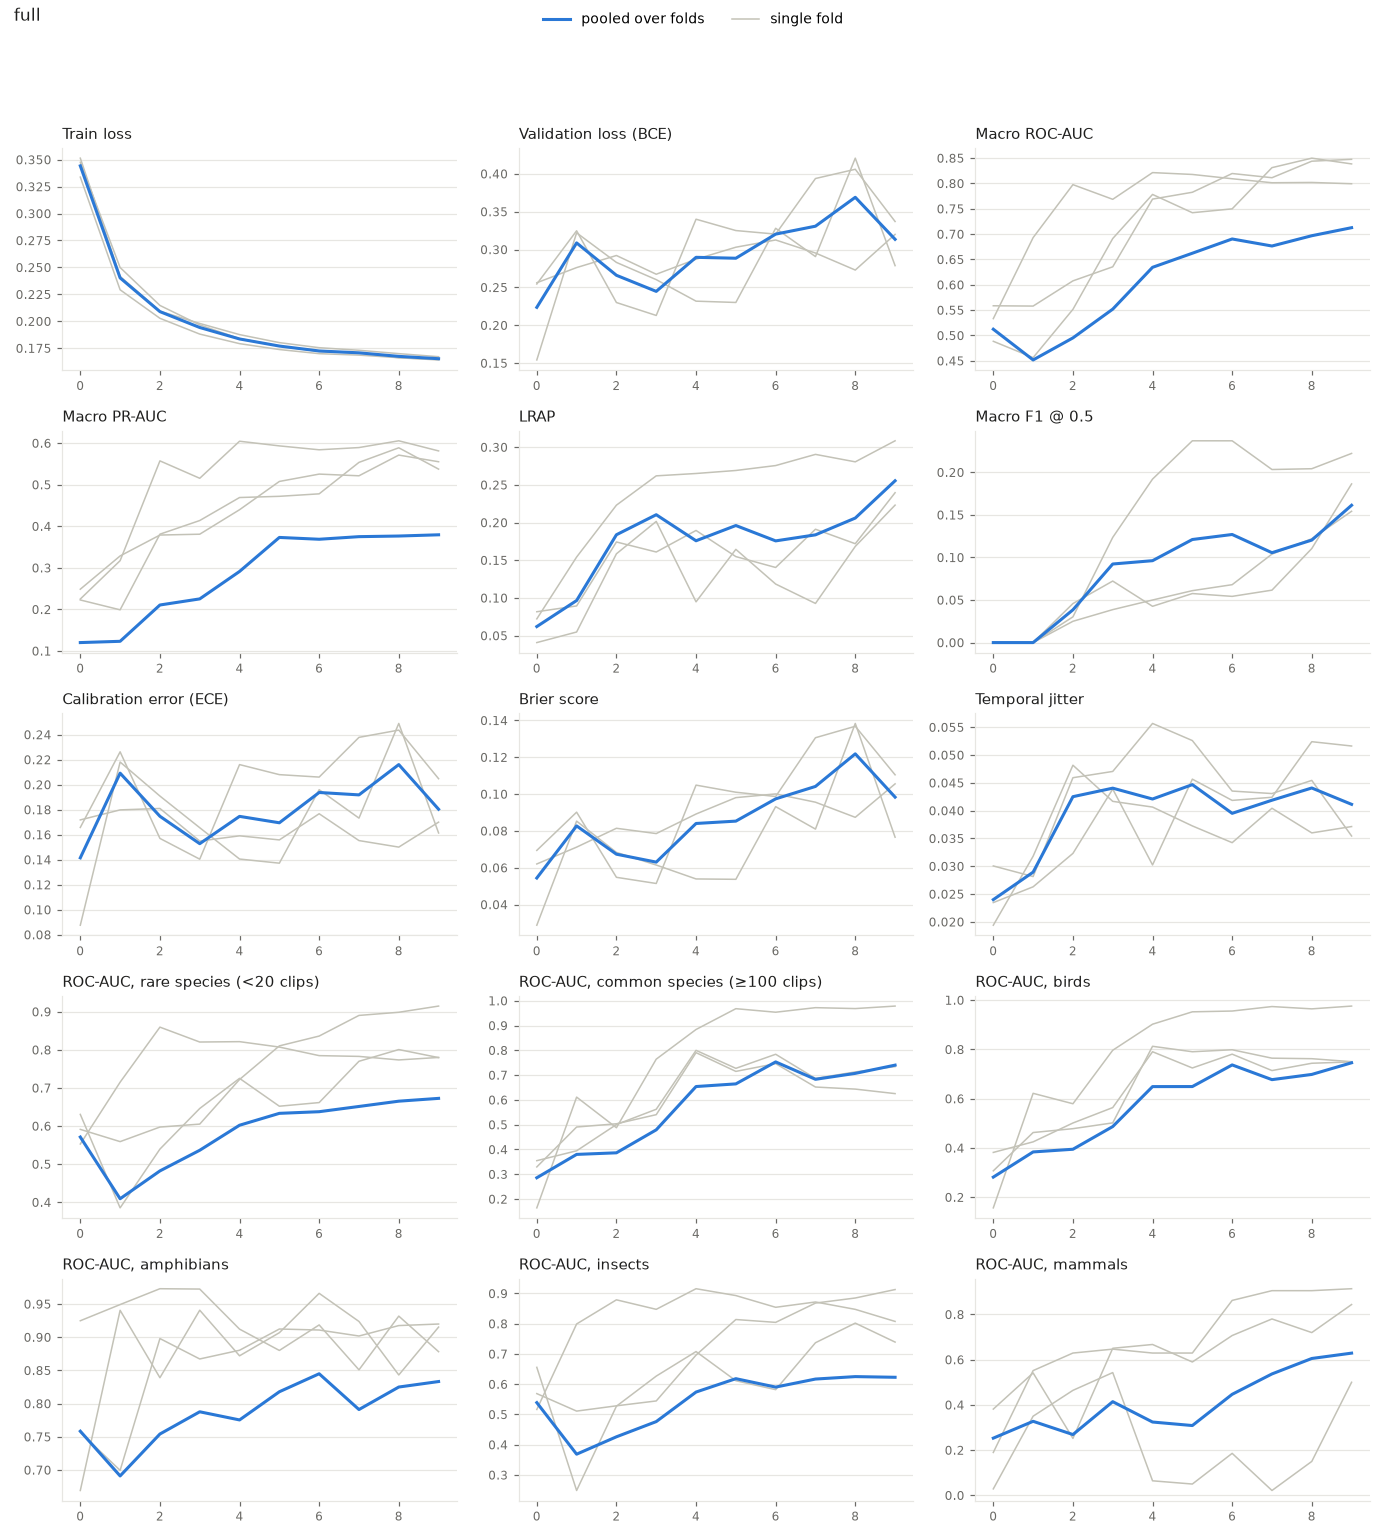
\includegraphics[width=0.9\linewidth]{curves_full.png}
\caption{\var{full}: per-fold (grey) and pooled (blue) curves for every
metric. Fold-local AUC (0.80--0.85 at the end) is well above the pooled
curve.}
\label{fig:curvesfull}
\end{figure}

\begin{figure}[H]
\centering
\begin{subfigure}{0.49\linewidth}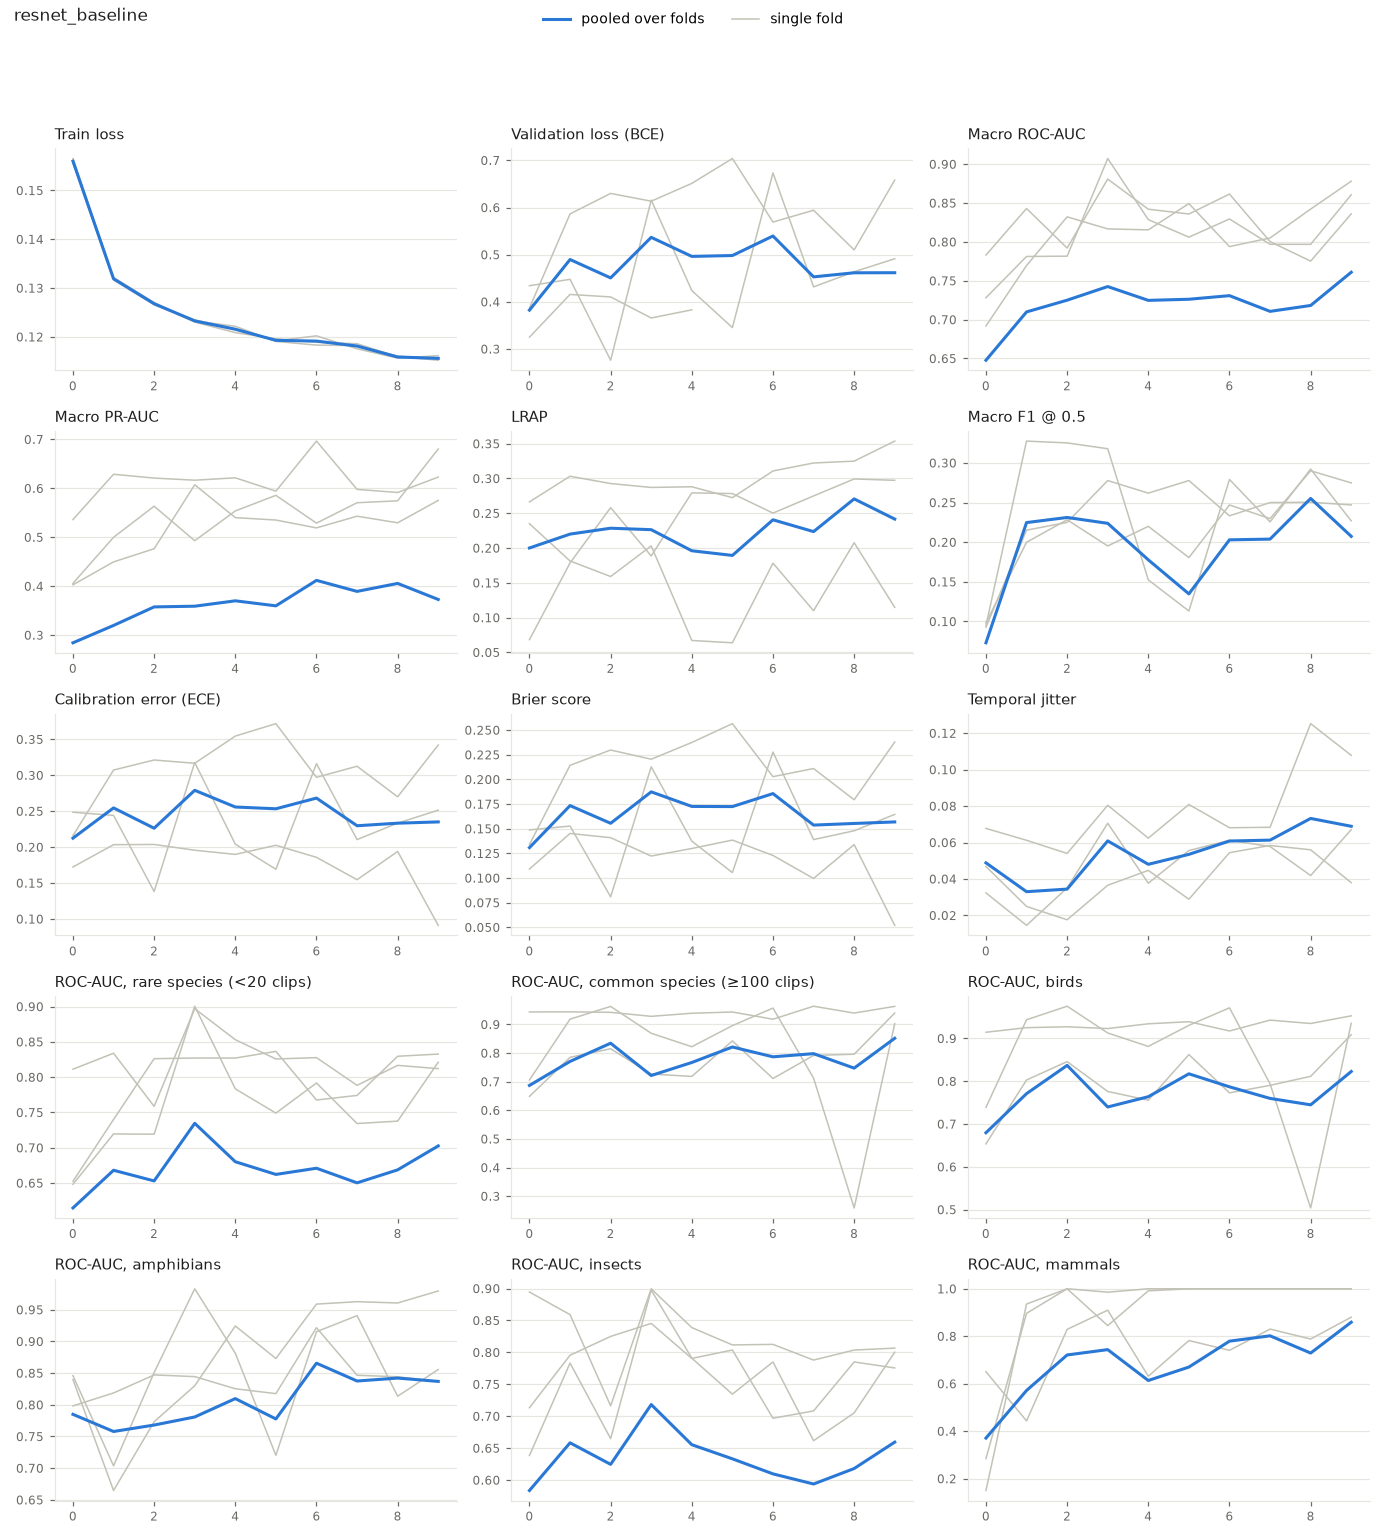
\includegraphics[width=\linewidth]{curves_resnet_baseline.png}\caption{\var{resnet\_baseline}}\end{subfigure}\hfill
\begin{subfigure}{0.49\linewidth}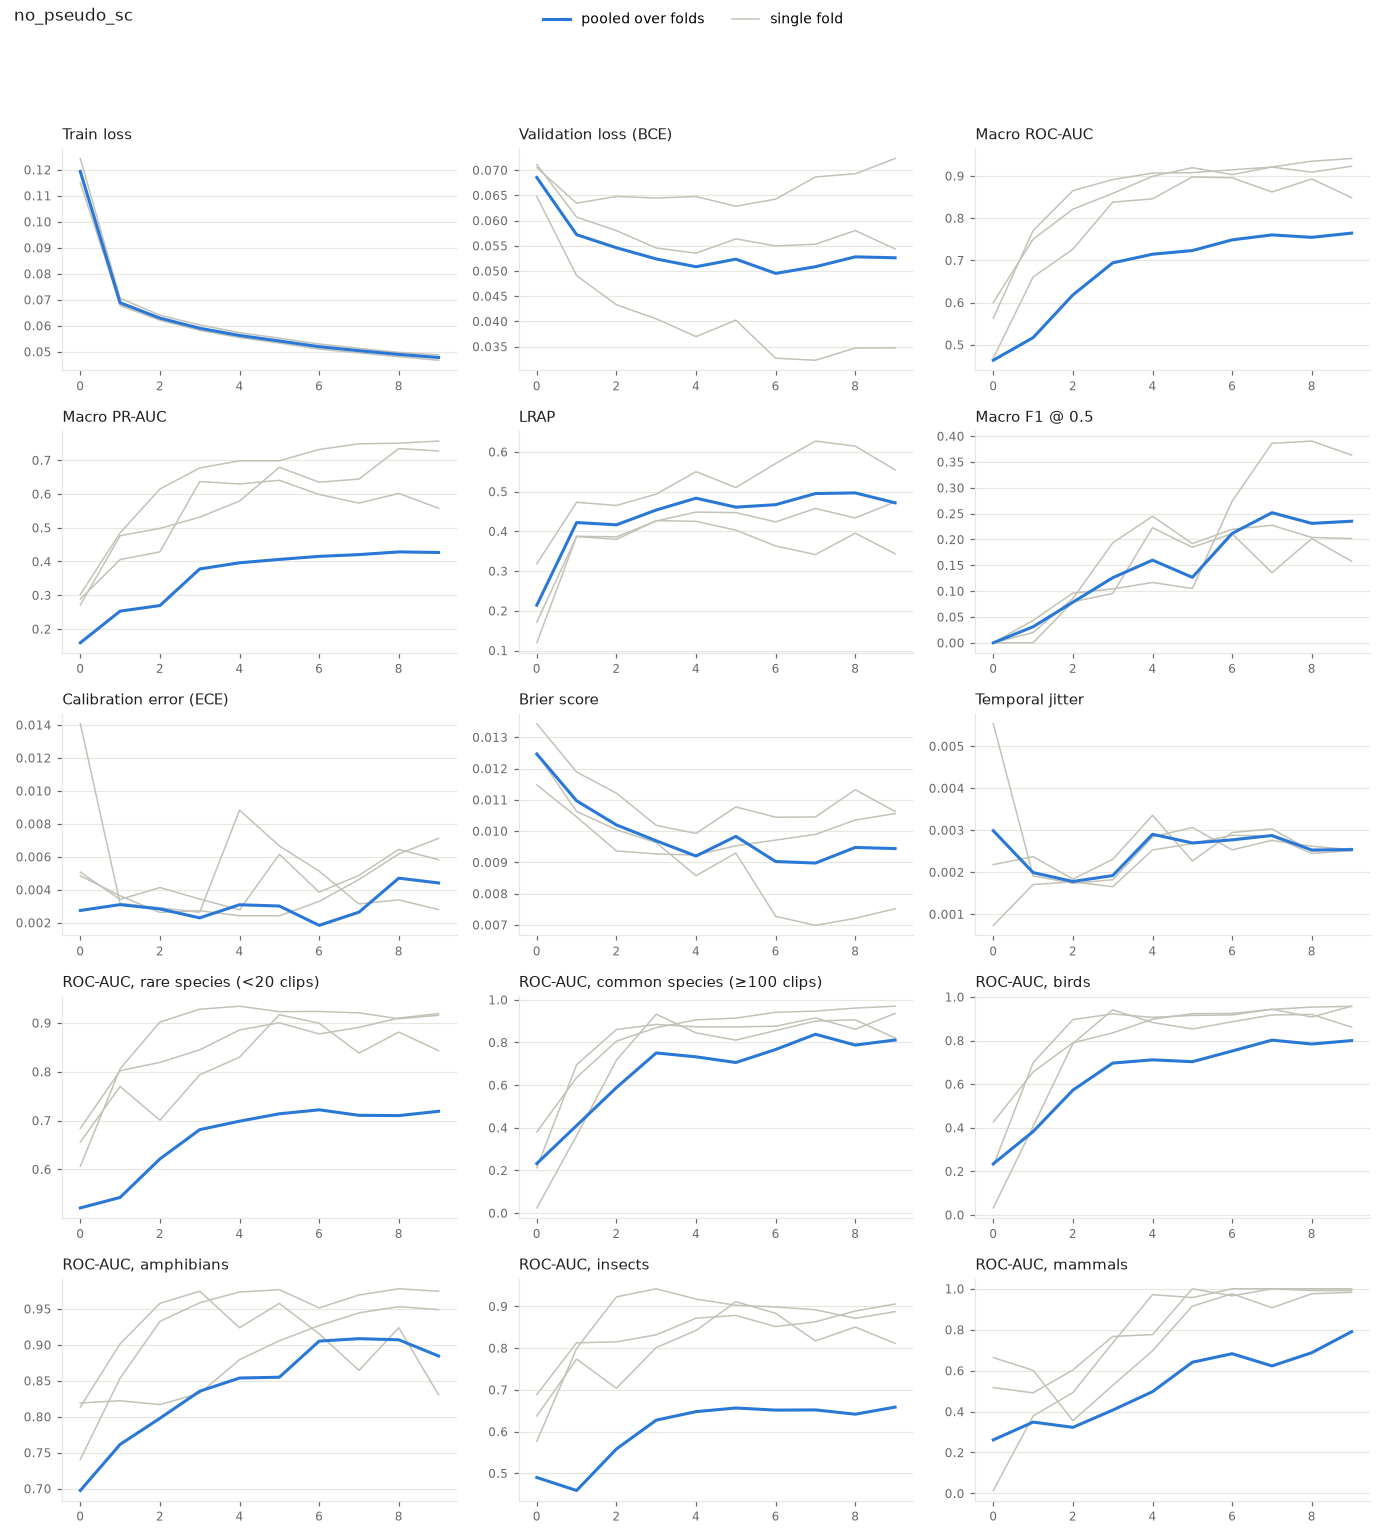
\includegraphics[width=\linewidth]{curves_no_pseudo_sc.png}\caption{\var{no\_pseudo\_sc}}\end{subfigure}
\caption{Per-fold and pooled curves for the two strongest trained models.}
\end{figure}

\subsection{Attention behaviour}
\label{sec:attn}
For 16 fixed labelled non-S22 validation windows per fold, the attention
weights over time and the class-activation map (the classifier applied to
every cell of the feature map) for the window's true species were recorded
after every epoch. We analysed the saved fold-0 tensors at the epoch with the
best fold-local non-S22 AUC. The fold-0 windows cover five classes (insect
sonotypes \texttt{47158son13} and \texttt{47158son10}, the caiman
\texttt{116570}, \texttt{516975} and the frog \texttt{1491113}).
\begin{itemize}
  \item \textbf{\var{full} (epoch 4).} The attention over the 10 time steps is
        close to uniform: the mean maximum weight is 0.120 against 0.100 for
        uniform, and the mean normalised entropy is 0.962. The average profile
        is $[0.028, 0.039, 0.116, 0.116, 0.115, 0.115, 0.116, 0.117, 0.118,
        0.120]$, so the first second is consistently down-weighted and the
        rest is flat. Profiles are similar across windows of different species
        (mean pairwise correlation 0.585). The predicted probability of the
        true species at that epoch averages 0.068 (median 0.027; range
        0.012--0.251), up from 0.035 at epoch 0.
  \item \textbf{\var{resnet\_baseline} (epoch 3).} By construction the
        attention is uniform (normalised entropy 1.0). Its probability for the
        true species averages 0.321 (median 0.177), up from 0.144 at epoch 0.
\end{itemize}

\begin{figure}[H]
\centering
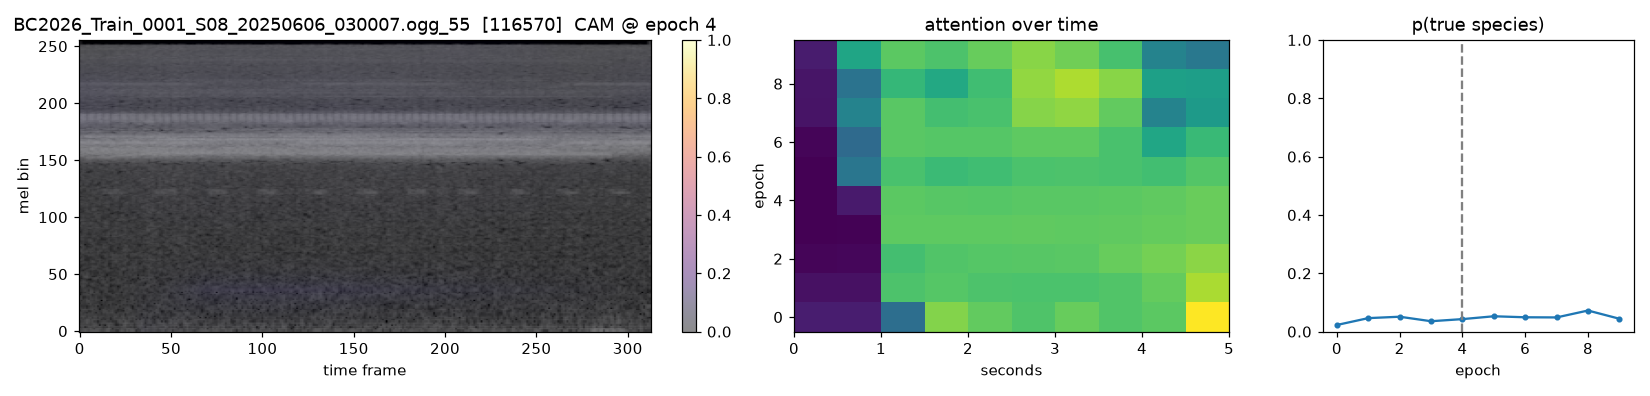
\includegraphics[width=\linewidth]{attn_full_116570.png}\\[2pt]
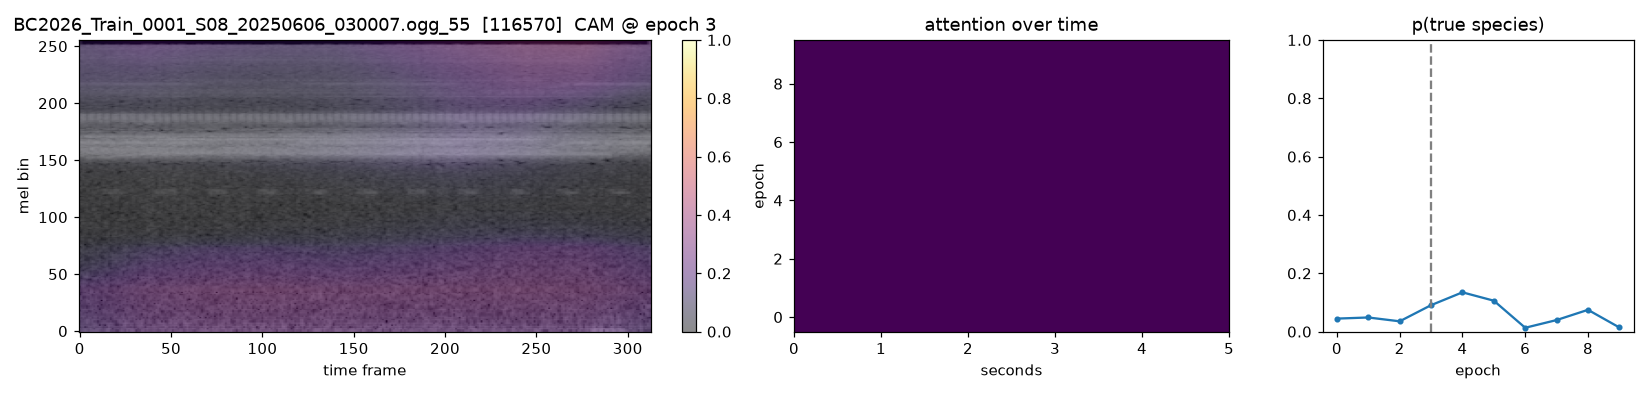
\includegraphics[width=\linewidth]{attn_res_116570.png}\\[2pt]
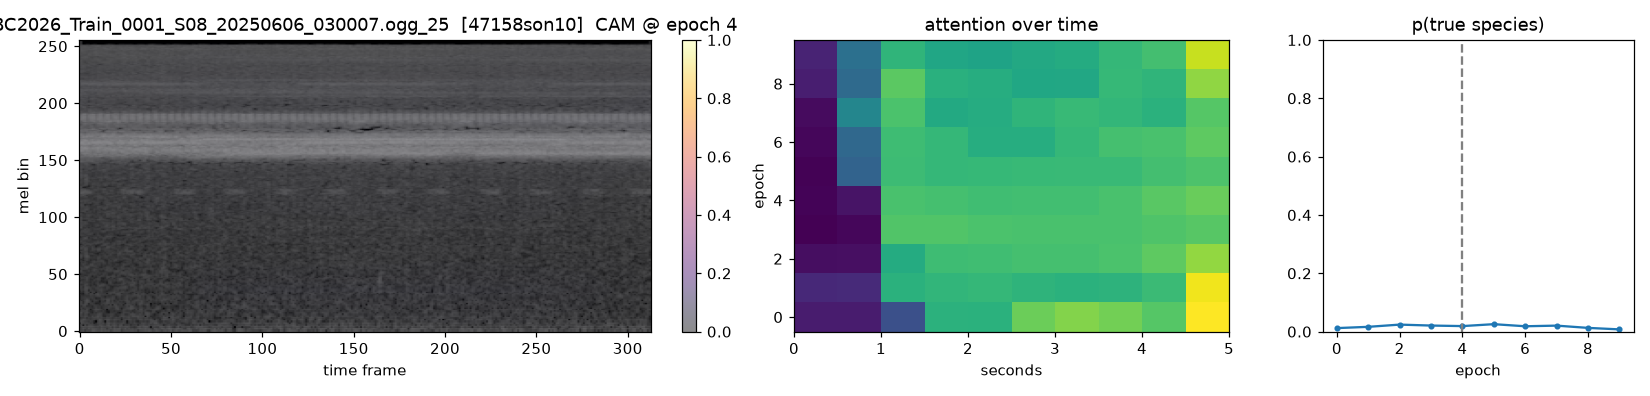
\includegraphics[width=\linewidth]{attn_full_47158son10.png}
\caption{Tracked windows (left: log-mel with class-activation overlay; middle:
attention over time per epoch; right: probability of the true species per
epoch, dashed line = best epoch). Top: \var{full} on a caiman
(\texttt{116570}) window. Middle: \var{resnet\_baseline} on the same window.
Bottom: \var{full} on an insect sonotype (\texttt{47158son10}). The
\var{full} attention has the same position-driven shape for both species: low
for the first second, highest in the last 0.5\,s at early epochs, and flat in
between.}
\label{fig:attn}
\end{figure}

% ===========================================================================
\section{Interpretation}
\label{sec:interp}

\subsection{How much can these rankings be trusted?}
The study is carefully controlled, but small. The primary metric averages 44
classes, evaluated on 16 files from 8 sites, and 26 of those classes are rare.
A single file can shift a class's AUC a lot. The bootstrap intervals
(Table~\ref{tab:boot}) are wide relative to most of the ablation effects, so
we group findings by strength:
\begin{itemize}
  \item \textbf{Robust:} the macro-AUC effects whose bootstrap interval
        excludes zero (mixup helps, mean beats GeM frequency pooling), and
        effects that are huge on metrics other than AUC and fit a clear
        mechanism. The latter are the calibration and ranking harm from
        pseudo-labelled soundscapes (ECE 0.184 vs 0.003, LRAP 0.221 vs
        0.477), the collapse of detection without soundscape data (F1 0,
        PR-AUC $-0.176$), the post-hoc gains, and the cost equivalence of all
        CNN variants (a measurement, not a sample).
  \item \textbf{Suggestive:} effects of 0.015--0.06 AUC that point in a
        consistent direction but whose interval just includes zero: the gain
        from removing pseudo-labelled soundscapes, the plain baseline beating
        \var{full}, and attention versus mean time pooling.
  \item \textbf{Noise-level:} effects under about 0.01 AUC (SpecAugment,
        single versus delta channels, rare upsampling on rare classes) and
        anything carried mainly by \textbf{Mammalia}. Mammal AUC ranges from
        0.4066 to 0.8447 across variants that differ only slightly, and its
        per-fold value swings between 0.02 and 0.91 from epoch to epoch.
\end{itemize}
Two further caveats apply. First, checkpoints were chosen on the same
validation folds that are scored, which inflates every absolute number
(although it affects all variants alike). Second, every variant got the same
short budget of 6{,}000 steps, which favours components that learn quickly
over ones that learn well eventually.

\subsection{Pseudo-labelled soundscapes are the main problem}
Removing the 24{,}000 pseudo-labelled soundscape windows is the single best
training change: macro AUC +0.060 (better in 97.4\% of bootstrap resamples), PR-AUC +0.069, LRAP +0.256, F1 +0.106, and ECE from
0.184 to 0.003. The pre-registered hypothesis expected the opposite, on the
grounds that unlabelled soundscapes are in-domain. We see three reasons it
went the other way.
\begin{enumerate}
  \item \textbf{The soft targets are not probabilities of presence.} Fused
        Perch scores plus site/hour prior logits give many classes moderate
        probabilities in every window. One batch in five trains the student to
        reproduce those values. The result is a model that predicts
        moderately high probabilities everywhere: validation BCE of
        0.22--0.37 and ECE of 0.15--0.22, against 0.05--0.12 BCE and ECE
        below 0.01 without that stream. The training loss of \var{full}
        levels off near 0.17 because soft targets have irreducible BCE.
  \item \textbf{The teacher is not much better than the student.} The
        Perch probe reaches only 0.711 macro AUC on these soundscapes and
        0.578 on rare species. Pseudo-labels cannot carry knowledge the
        teacher does not have, especially for the 28 classes with no focal
        clips and for sonotypes with no Perch mapping, which receive the prior
        alone or $-8$.
  \item \textbf{Ranking suffers with calibration.} LRAP, which ranks species
        within each window, nearly doubles without the stream (0.221
        $\rightarrow$ 0.477). That fits a picture in which the prior-dominated
        soft targets push the same site-typical species to the top of every
        window regardless of what is calling.
\end{enumerate}

\subsection{Distillation with stop-gradient slows learning}
In \var{full} the backbone never sees a classification gradient: it learns
only to imitate Perch embeddings, and a small head learns to read species from
those features. With 6{,}000 steps this is slow. Pooled AUC stays at or below
chance for three epochs and is still rising at epoch 9. Both alternatives that
let classification reach the backbone start much faster
(\var{resnet\_baseline}, \var{no\_distill}). The end result is mixed:
\var{no\_distill} is +0.015 AUC and +0.033 rare AUC better than \var{full},
but worse calibrated (ECE +0.041, which supports that hypothesis).
\var{distill\_no\_stopgrad} is $-0.017$ AUC and $-0.119$ on common species,
yet has a much higher F1 (+0.101). Our reading is that distillation adds a
\emph{regulariser and a delay}. At this budget the delay dominates, and the
cheaper end-to-end models win. Whether the distilled student overtakes them
with the notebook's 25 full epochs is the most important open question. It
also matters for cost, because distillation is free at inference.

\subsection{Simple beats sophisticated at this budget}
The pooled ResNet-18 baseline, with no attention, no GeM and no distillation,
is the second-best trained model (0.7571). It is better than \var{full} on
every taxon except Amphibia ($-0.010$), on rare (+0.042) and common (+0.073) species, on LRAP (+0.056)
and on F1 (+0.118). It is worse on calibration (ECE 0.226) and jitter (0.068),
because it also trains on the pseudo-labelled stream. The SED-head ablations
point the same way:
\begin{itemize}
  \item \textbf{GeM versus mean frequency pooling.} Mean pooling is better
        (+0.032 AUC, +0.084 F1, +0.069 LRAP), one of only two ablations whose
        bootstrap interval excludes zero. The prediction that insects and
        frogs, being narrow-band, would need GeM was not supported (Insecta
        +0.015 with mean pooling).
  \item \textbf{Attention versus mean time pooling.} Attention helps a little
        (mean pooling gives $-0.016$ AUC and $-0.011$ LRAP, supporting the
        hypothesis). The attention maps explain why the gain is small: they
        are nearly uniform and mostly encode \emph{position}, down-weighting
        the first second of every window (Section~\ref{sec:attn}). The
        position effect may come from zero-padding at the window edge in the
        convolutional receptive field. The model is not yet acting as an event
        detector.
  \item \textbf{Clip versus frame-max heads.} Frame-max alone matches the
        blend (0.7145 versus 0.7142) and is more over-confident (ECE +0.036,
        supported). Clip-only is worse (0.7050). The 50/50 blend mainly buys
        calibration.
\end{itemize}

\subsection{Delta channels are not worth it}
Dropping the delta and delta-delta channels changes macro AUC by +0.009,
which is within noise, and Insecta by only $-0.002$. That technically
``supports'' the hypothesis, but the effect is negligible. It also gives the
cheapest model (5.65 versus 5.91 GFLOPs, 0.73 versus 0.79\,ms on GPU, 80.8
versus 81.9\,ms on CPU) and the start of every Pareto frontier. The idea that
temporal derivatives help with repetition-rate-defined insect and frog calls
is not supported. A ResNet's first layers can learn such derivatives from
log-mel alone.

\subsection{Mixup and labelled soundscapes are essential}
Removing mixup costs the most AUC of any training change ($-0.051$, the only
harmful change whose bootstrap interval excludes zero) and lowers every taxon. Removing soundscape data costs $-0.049$ AUC, $-0.176$ PR-AUC,
$-0.162$ LRAP, F1 down to zero, Amphibia $-0.257$ and rare $-0.086$. Yet it
\emph{raises} common-species AUC (+0.102). Frogs and insects are recorded
mainly in soundscapes, and soundscape backgrounds differ greatly from focal
recordings. A model trained only on focal clips stays good at ranking common
birds but is not calibrated for the deployment domain: no probability crosses
0.5. Focal--soundscape mixup and the small labelled-soundscape stream (about
630 windows per fold) are what adapt the model to the field.

\subsection{The free wins: post-processing}
Every post-hoc step that uses context the network cannot see helped, and they
stack:
\begin{itemize}
  \item \textbf{Site/hour prior:} AUC +0.020, LRAP +0.175, ECE 0.184
        $\rightarrow$ 0.006, Mammalia +0.172. Where and when a recording was
        made strongly constrains which species can be present.
  \item \textbf{Taxonomy smoothing:} rare +0.063, Amphibia +0.073, Insecta
        +0.082. Rare species borrow evidence from relatives in the same genus.
  \item \textbf{Temporal smoothing:} jitter 0.044 $\rightarrow$ 0.012 and
        PR-AUC +0.031. Calls last longer than 5\,s and soundscape choruses
        persist.
  \item \textbf{All three:} AUC 0.8407 (+0.127), rare 0.8335, Insecta 0.8558,
        Amphibia 0.9139, jitter 0.0013, ECE 0.0062. The ``free'' lookup and
        averaging steps contribute more than any architectural component.
\end{itemize}
One caution applies. Folds are grouped by file, not by site, so the prior for
a validation file is fit partly on other recordings from the \emph{same}
sites. The gain therefore reflects deployment at sites with labelled history.
At a brand-new site the site and site-hour terms shrink back to the hourly and
global priors, and the benefit would be smaller.

\subsection{The teacher alone: good on birds, poor elsewhere, expensive}
The Perch probe is the best ranker of common species (0.904) and birds
(0.897), as expected from a model trained on huge bird collections. It is the
worst on rare species (0.578, against a predicted rise), insects (0.491),
calibration (ECE 0.356) and jitter, and second-worst on LRAP (0.139). Its curve plateaus after one
epoch, so the frozen features, not the training budget, limit it. It also
needs a GPU (2.57\,ms per window, no CPU path). For a CPU-only field station
it is not an option, and its knowledge reaches the student only where it is
strong (birds).

\subsection{Cost: the architecture choices are free}
The most practical result is that \emph{none of the studied components change
inference cost meaningfully}. All CNN variants differ by less than 4\% in CPU
time (80.8--83.6\,ms per window, single thread) and by less than 8\% in
GFLOPs. Distillation, pseudo-labels, mixup, SpecAugment and upsampling are
training-time only, and the post-hoc steps are table lookups and averages.
One CPU thread processes a 5\,s window in about 82\,ms, i.e.\ 61 seconds of
audio per second. Four threads take about 22\,ms per window, roughly
227$\times$ real time, which is ample headroom for many recorders per box. The
cost question is decided by the backbone (ResNet-18 here), and every component
choice should be made purely on quality.

\subsection{Pooled versus fold-local scoring}
Fold-local AUCs (0.70--0.94) are far above the pooled out-of-fold scores
(0.66--0.77). Part of the gap is selection bias, since each checkpoint was
picked on its own fold. The rest comes from pooling: the three fold models
produce scores on different scales, and a single ranking across them
penalises that inconsistency. Deployment uses one model with one score scale,
so the pooled number is closer to deployment behaviour for threshold-free
ranking. Even so, the per-fold numbers show that within one model the ranking
of species is considerably better than the pooled score suggests.

\subsection{What the failed hypotheses teach}
The 13 supported hypotheses mostly concern cheap, well-understood components:
mixup, soundscape data, SpecAugment, time attention, smoothing and priors. The
8 unsupported ones are distillation helping
rare species, pseudo-labelled soundscapes helping, Perch beating the student
on rare species, GeM helping narrow-band taxa, the pooled baseline being worse
than the SED head, the clip/frame blend beating either head, Perch-localised
focal targets helping precision, and stop-gradient being harmless. Five of the eight are about using the
teacher (distillation, stop-gradient, Perch-localised targets, pseudo-labelled
soundscapes, Perch on rare species): every idea that relies on the teacher's
knowledge failed to pay off at this budget.

% ===========================================================================
\section{Limitations}
\begin{enumerate}
  \item \textbf{Small evaluation set:} 192 windows, 16 files, 8 sites, 44
        scorable classes and a single seed. Mammalia and other low-count
        groups are especially unstable.
  \item \textbf{Optimistic selection:} the checkpoint epoch is chosen on the
        scored validation fold, using a criterion (all windows, S22 included)
        that differs from the reported metric (non-S22).
  \item \textbf{Short budget:} 10$\times$600 steps, constant learning rate,
        and only 3 of 5 folds trained. Slower-learning components are
        disadvantaged, and \var{full} had not converged.
  \item \textbf{One change at a time:} interactions were not tested. In
        particular the obvious combination (no pseudo-soundscapes, mean
        frequency pooling, single channel, plus post-processing) was not
        trained.
  \item \textbf{Site leakage in priors:} site/hour priors and pseudo-label
        fusion use other files from the same sites.
  \item \textbf{Shared-GPU timing:} training times were measured with three
        concurrent runs, so epoch times reflect lane contention. Inference
        timings were measured on an idle machine.
  \item \textbf{Augmentation change:} waveform gain and noise augmentation
        from the original notebook were dropped when spectrograms were
        precomputed.
\end{enumerate}

% ===========================================================================
\section{Recommendations}
\label{sec:recommend}
For a CPU-only on-site monitor, the evidence supports:
\begin{enumerate}
  \item A ResNet-18 trained end-to-end on single-channel log-mel, with the
        classification gradient reaching the backbone, mean frequency pooling,
        and the attention or pooled head.
  \item Training \emph{with} mixup (focal--focal and focal--soundscape) and
        labelled soundscapes, and \emph{without} the pseudo-labelled
        soundscape stream, at least until its targets are recalibrated (for
        example by sharpening, thresholding or confidence weighting).
  \item The three post-processing steps (site/hour prior, temporal
        smoothing, taxonomy smoothing), which cost nothing to run and gave the
        largest single gain in the study.
  \item Before deployment, confirming the combined configuration with all 5
        folds, several seeds, the full training budget and site-grouped
        validation. This would also settle whether distillation pays off once
        training is long enough.
\end{enumerate}
Such a model runs at about 61$\times$ real time on one CPU thread.

% ===========================================================================
\section{Conclusion}
We set out to find the cheapest model that still performs well for
continuous, on-site acoustic monitoring of the Pantanal's birds, frogs,
insects and mammals. Under a fixed, short training budget, the elaborate
distilled SED network (0.7142 macro ROC-AUC) was beaten by a plain ResNet-18
(0.7571) and by the same network without pseudo-labelled soundscapes
(0.7742). The latter also cut calibration error by a factor of about 57.
Mixup and labelled soundscapes are essential. Delta channels, GeM pooling and
Perch-based supervision did not earn their place. Every component is free at
inference (about 82\,ms per window on one CPU thread), so the choice should be
made on quality. Free post-processing with site/hour priors, temporal
smoothing and taxonomy smoothing raised macro ROC-AUC to 0.8407. With an
evaluation set of 16 files, the large effects are trustworthy and the small
ones are not. The clear next step is to train the combined simple
configuration longer, on all folds, with site-grouped validation.

% ===========================================================================
\section*{Acknowledgements and Attribution}
The SED head, Perch distillation with stop-gradient, pseudo-labelling system,
site/hour priors and taxonomy smoothing are adapted from nina2025's Kaggle
notebook ``BirdCLEF~2026 EoS.9''~\cite{nina2025}. That notebook builds on
tuckerarrants' distilled-SED and waveform-cache datasets and the BirdCLEF~2025
first-place SED design by nikitababich. Perch~v2 is by Google
DeepMind/Google Research~\cite{perch}. Data are from the BirdCLEF~2026
competition~\cite{birdclef}.

\begin{thebibliography}{9}
\bibitem{nina2025} nina2025. \emph{BirdCLEF 2026 EoS.9} (Kaggle notebook,
sections Model\_1 and Model\_22).
\url{https://www.kaggle.com/code/nina2025/birdclef-2026-eos-9}
\bibitem{birdclef} BirdCLEF 2026 competition data (Kaggle / LifeCLEF), Pantanal
focal recordings, soundscapes and taxonomy.
\bibitem{perch} Google DeepMind / Google Research. Perch~v2 bioacoustics
model.
\bibitem{he2016} K.~He, X.~Zhang, S.~Ren, J.~Sun. Deep residual learning for
image recognition. \emph{CVPR}, 2016.
\bibitem{park2019} D.~S.~Park et al. SpecAugment: a simple data augmentation
method for automatic speech recognition. \emph{Interspeech}, 2019.
\bibitem{hinton2015} G.~Hinton, O.~Vinyals, J.~Dean. Distilling the knowledge
in a neural network. \emph{NIPS Deep Learning Workshop}, 2015.
\bibitem{zhang2018} H.~Zhang, M.~Cisse, Y.~N.~Dauphin, D.~Lopez-Paz. mixup:
beyond empirical risk minimization. \emph{ICLR}, 2018.
\end{thebibliography}

\end{document}
